\documentclass[11pt,a4paper]{article}

\usepackage[T1]{fontenc}
\usepackage[utf8]{inputenc}
\usepackage{lmodern}
\usepackage{geometry}
\usepackage{amsmath}
\usepackage{booktabs}
\usepackage{enumitem}
\usepackage{float}
\usepackage{hyperref}
\usepackage{graphicx}
\usepackage{array}
\usepackage{tabularx}

\geometry{margin=2.3cm}
\setlist[itemize]{leftmargin=*}
\setlist[enumerate]{leftmargin=*}
\newcolumntype{L}[1]{>{\raggedright\arraybackslash}p{#1}}
\newcolumntype{Y}{>{\raggedright\arraybackslash}X}

\title{SPPA: A Runtime Contract and Preliminary Prototype for Semantic Primitive Proxy Actors in UAV Digital Twins}
\author{Authors omitted for review}
\date{}

\begin{document}

\maketitle

\begin{abstract}
Telemetry-driven UAV digital twins can receive object-level perception messages
that are too sparse to render as recognizable actors directly. This creates a
semantic telemetry-to-actor gap: the perception stream may provide a class,
confidence, pose estimate, bounding region, or footprint, while the rendering
layer needs an immediately visible object with meaningful occupied volume and
predictable cost. This paper specifies and preliminarily instruments Semantic
Primitive Proxy Assembly (SPPA), a bounded representation contract for compiling
semantic labels into low-polygon proxy actors made of boxes, cylinders,
ellipsoids, cones, and tori. SPPA is not a planner occupancy map, not a
certified detect-and-avoid layer, not a 3D reconstruction method, and not a
replacement for video. It is a proposed actor-representation layer within a
larger UAV digital-twin pipeline. The current artifacts include a legacy
seven-class OBJ/MTL debug prototype, a bounded-label Python resolver/fallback
path, a Python \texttt{SPPA-DESC-0.2}/\texttt{SPPA-UPD-0.2} descriptor and
update-packet implementation, and a native Unreal backend-switch plus
descriptor-ingestion smoke test, Editor-Cmd actor microbenchmark, and component
payload replay; they do not yet consume live YOLO tracks inside Unreal or
provide VR/user validation. We provide the runtime contract, descriptor schema,
semantic compiler specification, evidence-status table, preliminary local
stress tests against text/image-to-3D generators, lifecycle timing measurements,
descriptor/update-packet measurements, a packaged internal Unreal render
benchmark,
and an evaluation roadmap. The artifacts do not yet establish dense VR frame
rate, operator readability, fallback behavior, comparative bandwidth advantage,
or end-to-end UAV operation.
\end{abstract}

\section{Motivation}

The target semantic-telemetry UAV visualization architecture replaces continuous video transmission with lightweight semantic
telemetry. The UAV does not transmit every pixel of the camera stream; it
transmits object-level meaning: class label, confidence, position, timestamp,
and approximate geometry. The ground station reconstructs the operational scene
inside a Cesium-enabled Unreal Engine digital twin for a remote pilot wearing VR
goggles.

This architecture creates a practical rendering problem. A detector may report
many classes: people, cyclists, cars, trucks, animals, vegetation, poles,
barriers, construction machinery, unknown obstacles, and rare objects. A digital
twin cannot realistically maintain a complete, manually curated 3D asset library
for every object that might appear during real-world UAV operation. Even if a
large library is available, asset retrieval, licensing, semantic matching,
level-of-detail management, and runtime loading remain operational problems.

Modern image-to-3D and text-to-3D models address a different objective. They are
designed to create visually rich 3D assets from images or prompts. This is
valuable for content creation, simulation authoring, games, and design. However,
remote UAV piloting has a different priority: a detected object must appear in
the pilot's synthetic world under a predictable rendering budget. In the current
local debug path, SPPA emits coarse proxy meshes in milliseconds; this is a
measured prototype property, not a claim that every neural generator necessarily
requires seconds under every configuration.

\section{Core Idea}

The proposed system performs semantic primitive proxy generation. The key claim
is simple:

\begin{quote}
For telemetry-driven UAV visualization, the digital twin may not need to
reconstruct the true mesh of every detected object. The hypothesis is that a
low-latency, low-polygon, semantically recognizable volume can preserve enough
operational context to justify further operator-facing evaluation.
\end{quote}

Instead of producing a detailed mesh, the system assembles predefined geometric
primitives into a proxy structure. The proxy is not only selected by class name;
it is selected by a lightweight semantic and morphological interpretation of
that class. If the detector reports \texttt{cow}, the system can infer that the
object is an animal, a mammal, and a quadruped. That immediately constrains the
proxy to include a body volume, a head volume, four legs, and an orientation
hypothesis. If the detector reports \texttt{truck}, the system can infer a long
vehicle body, a cab, wheels, and an elongated footprint. The silhouette then
adjusts the proportions: a long truck and a short truck share the same semantic
template, but the cargo body is scaled differently. For example:

\begin{itemize}
    \item a cow may be represented by ellipsoids for body and head, cylinders
    for legs, and cones for horns;
    \item a cyclist may be represented by two torus wheels, a simple bicycle
    frame, and a human torso/head proxy;
    \item a tree may be represented by a cylinder trunk and clustered green
    volumes;
    \item a car or truck may be represented by boxes and wheel tori;
    \item a bush may be represented by overlapping green ellipsoids.
\end{itemize}

The exact geometry is intentionally crude. Its purpose is to encode:

\begin{itemize}
    \item approximate occupied volume;
    \item object class recognizability;
    \item spatial location;
    \item scale relative to the scene;
    \item extremely low rendering complexity.
\end{itemize}

Scale and proportion adaptation are only partially implemented, but the
implemented vehicle path is no longer a root-scale deformation of the whole
actor. For supported vehicle archetypes, explicit metric dimensions drive a
semantic part-layout rule: a longer truck extends the cargo/body span and axle
placement while cab and wheel dimensions remain bounded by their own part
priors. The Unreal update path likewise rejects shape updates that contain only
a new global scale and requires replacement part parameters for
\texttt{shape\_param\_update}. The generator now also supports a calibrated
mask/bbox route: if an explicit image-to-ground scale is supplied, the oriented
footprint can derive metric length/width and drive the same parametric part
layout. Without that calibration, masks remain image-space evidence only.
Real observed-silhouette part fitting remains unevaluated. Non-vehicle
archetypes still use template priors or coarse fallback dimensions. This is
important for UAV piloting: when flying over an object, the relevant question
is not whether the rendered actor is visually beautiful, but whether its
occupied volume and part semantics are approximately correct for navigation and
operator interpretation. That claim remains a validation target until the
planned volume-error and operator studies are completed.

\begin{figure}[t]
\centering
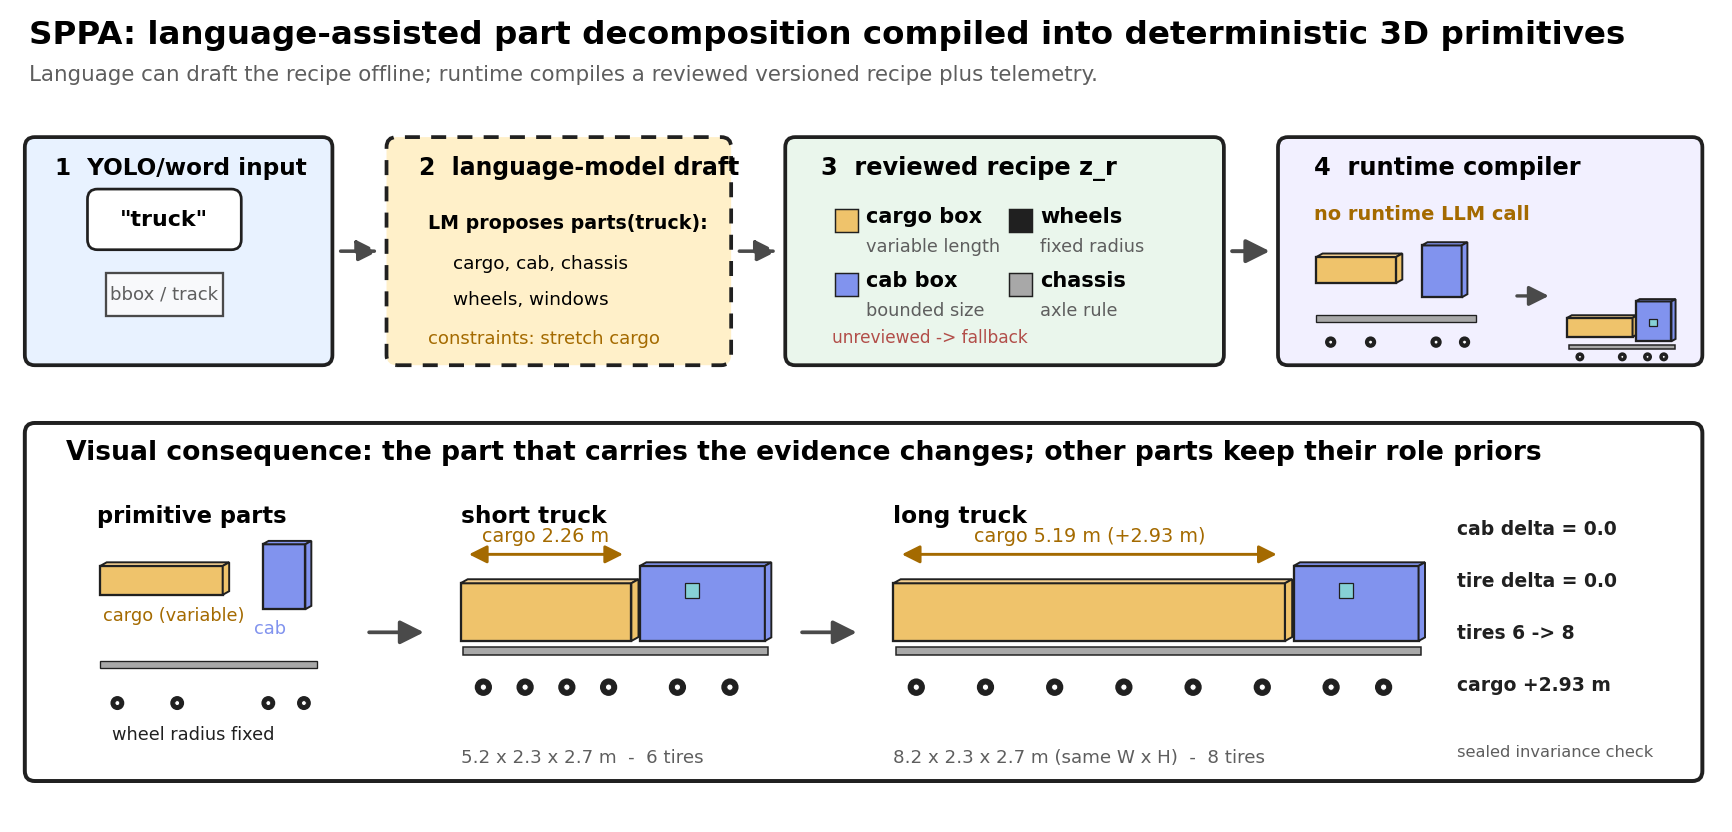
\includegraphics[width=\linewidth]{figures/sppa_language_to_parts_to_3d_v17.png}
\caption{SPPA language-to-parts-to-geometry recipe example. A language
model, ontology tool, or human author may draft candidate parts and constraints
offline, but runtime uses a reviewed versioned recipe \(z_r\), not a language
model or neural mesh generator. The truck example shows the intended chain
explicitly: semantic label or word, offline part proposal, reviewed part-role
recipe, primitive constraints, and deterministic assembly with role-specific scale
rules rather than global object scaling.}
\label{fig:sppa-flow}
\end{figure}


\section{Operational Scope and Non-Claims}

The contribution claimed in this manuscript is intentionally narrow. SPPA is a
runtime representation contract for intended display proxy actors, not the flight
system itself. The surrounding UAV visualization stack provides the broader telemetry, networking, tracking,
Unreal/Cesium integration, and VR interface context. SPPA addresses only the
question of how an object-level semantic state can be represented visually when
a curated asset is unavailable, too costly, or insufficiently matched to the
observed object.

The testable claim is therefore:

\begin{quote}
For telemetry-driven UAV digital twins, track-persistent semantic primitive
actors may provide a bounded, uncertainty-aware, intended display obstacle volume
when image evidence is missing, degraded, or insufficient for high-fidelity
asset generation.
\end{quote}

This paper does not claim evaluated UAV/VR teleoperation performance. It also
does not claim planning-level risk guarantees, collision avoidance, network-efficiency benefit, or
operator benefit. Those are evaluation targets, not results.

SPPA's novelty is not procedural geometry itself; it is the telemetry-to-runtime-rendering contract with track persistence, uncertainty metadata, and optional fallback beside curated asset spawning.

\section{Contributions}

This manuscript is framed as a runtime-contract paper with preliminary
instrumentation. The contributions are separated by evidence status:

\begin{enumerate}
    \item \textbf{Implemented template and fallback artifacts.} A seven-class fixed-template debug
    prototype exports SPPA-style proxy meshes through an OBJ/MTL batch path.
    This artifact demonstrates visual style and local generation timing only;
    it does not implement live telemetry ingestion. Descriptor-level scale
    evidence and optional native Unreal descriptor ingestion are implemented,
    including actor-level pose and shape update smoke tests and a packaged
    synthetic render benchmark up to 100 objects; dense VR/live runtime behavior
    remains unevaluated. Fallback behavior is smoke-tested in
    Python/Unreal but not evaluated operationally.
    \item \textbf{Implemented Python descriptor/update contract.} The current
    generator emits SPPA-DESC/SPPA-UPD v0.2 artifacts with an explicit semantic
    resolver contract, bbox/mask/world-pose evidence, yaw provenance and
    ambiguity, scale source, material source, primitive parts, cost fields, and
    scheduler metadata. A
    companion \texttt{SPPA-UPD-0.2} packet separates create/regenerate payloads
    from per-frame pose or shape updates. Unreal now includes an optional
    native descriptor-ingestion path that constructs primitive components from
    descriptor \texttt{parts[]} and an update-packet path for
    pose/no-op/shape updates while preserving the existing asset backend as the
    default.
    \item \textbf{Preliminary measurements.} We report local timing and mesh
    complexity measurements for the current template path, descriptor/update
    packet timing and size measurements, a track-lifecycle replay over
    available obstacle logs, a packaged internal Unreal render benchmark, and
    stress tests against selected fast text/image-to-3D generators under a
    constrained PyTorch allocator budget. These are preliminary operating-point
    measurements, not statistical or end-to-end UAV/VR validation.
    \item \textbf{Specified runtime contract.} We define the SPPA descriptor,
    semantic-to-archetype compiler, part-graph representation, uncertainty
    metadata, yaw ambiguity handling, and uncertainty-marked generic fallback
    requirements.
    \item \textbf{Positioning and evaluation protocol.} We position SPPA as a
    track-persistent semantic actor representation, distinct from primitive
    shape theory, occupancy mapping, curated asset loading, and neural 3D asset
    generation. We provide falsifiable hypotheses and a planned evaluation
    roadmap for the missing Unreal, geometry, operator, fallback, and bandwidth
    evidence.
\end{enumerate}

\section{Research Question and Hypotheses}

The scientific question behind SPPA is not whether primitive geometry can look
realistic. It is:

\begin{quote}
What is the minimum semantic-volumetric representation that preserves enough
operational information for a future remote UAV visualization interface?
\end{quote}

This question leads to falsifiable hypotheses. None of H1--H5 is claimed as
evaluated by the current prototype:

\begin{description}[leftmargin=1.2cm,style=nextline]
    \item[H1 latency.] SPPA is designed to reduce detection-to-visible-actor
    latency relative to runtime asset loading or neural generation. Required
    baselines are box, capsule, low-poly asset loading, and image-to-3D; primary
    metrics are P50/P95 latency, triangles, and descriptor bytes. This hypothesis
    is unevaluated in the current artifact.
    \item[H2 recognition.] SPPA is hypothesized to increase class-family
    recognition relative to generic boxes, capsules, or label billboards at
    comparable rendering cost. Required baselines are 3D box,
    capsule/ellipsoid, and billboard label; primary metrics are recognition
    accuracy, response time, and confusion matrix. A user study is absent.
    \item[H3 proportionality.] SPPA is designed to preserve footprint and
    occupied volume better than fixed-scale templates when object proportions
    vary. Required baselines are fixed template, bbox-only scale, and curated
    low-poly asset; primary metrics are BEV IoU, volume error, and height error.
    This hypothesis is unevaluated in real or simulated UAV detections.
    \item[H4 dense runtime.] SPPA is hypothesized to scale to dense VR scenes
    with more predictable rendering cost than detailed mesh assets. Required
    baselines are boxes, capsules, low-poly assets, and detailed meshes; primary
    metrics are FPS, CPU/GPU frame time, and draw calls. A dense-runtime
    benchmark is absent.
    \item[H5 fallback.] SPPA is designed to fall back to uncertainty-marked
    generic volumes under uncertain class, scale, silhouette, or yaw evidence.
    Required baselines are no rendering, box, and uncertainty volume; primary
    metrics are containment rate, false-confidence events, and operator
    interpretation. A fallback-interpretation study is absent.
\end{description}

\section{A Different Runtime Contract from 3D Generation}

Recent 3D generative methods have advanced rapidly. DreamFusion introduced a
text-to-3D optimization approach using a pretrained 2D diffusion model and score
distillation sampling \cite{poole2022dreamfusion}. Magic3D improved quality and
speed with a coarse-to-fine strategy, but still reports mesh creation times on
the order of tens of minutes \cite{lin2022magic3d}. Point-E reduced generation
time substantially, producing point clouds in roughly 1--2 minutes on a single
GPU, while explicitly trading quality for speed \cite{nichol2022pointe}.
Shap-E further generates implicit 3D functions from text or image conditions in
a matter of seconds \cite{jun2023shape}. In this manuscript, Point-E and Shap-E
are treated as legacy direct text/tag baselines, not as the strongest 2026
image-conditioned asset generators.

More recent feed-forward image-to-3D methods are faster. TripoSR reports
single-image mesh reconstruction in under 0.5 seconds \cite{tochilkin2024triposr}.
InstantMesh reports diverse single-image 3D assets within approximately 10
seconds \cite{xu2024instantmesh}. Stable Fast 3D reports textured mesh
reconstruction from a single input image in approximately 0.5 seconds
\cite{stability2024sf3d,sf3d2024}. LGM, CRM, and Unique3D are also relevant fast
image-conditioned generators \cite{tang2024lgm,wang2024crm,wu2024unique3d}.
TRELLIS/TRELLIS.2 and Hunyuan3D 2.x focus on high-quality, versatile, textured
3D asset generation using large-scale latent or diffusion architectures
\cite{xiang2024trellis,xiang2025trellis2,zhao2025hunyuan3d,hunyuan2025hunyuan3d21}.
Recent benchmark work, including HY3D-Bench and P3D-Bench, also makes clear that
a credible SOTA ranking needs shared reference inputs, explicit metrics, and
part/structure evaluation rather than a local qualitative grid assembled from
heterogeneous input types \cite{hunyuan2026hy3dbench,yang2026p3dbench}.

These methods are impressive, but they are not optimized for the same operating
point. In UAV VR teleoperation, several constraints become dominant:

\begin{itemize}
    \item \textbf{Per-object latency:} dynamic detections must appear in the
    digital twin under a fixed runtime budget; neural asset generation may be
    unsuitable unless it is precomputed, cached, or wrapped in its own
    tracking/fusion layer.
    \item \textbf{Scene density:} the scene may contain hundreds of people,
    animals, vehicles, trees, or temporary obstacles.
    \item \textbf{VR frame rate:} the pilot interface must remain stable and
    comfortable; geometric complexity must be predictable.
    \item \textbf{Input availability:} a clean cropped image suitable for
    image-to-3D generation may not be available under poor visibility, motion
    blur, compression, occlusion, or low-confidence detection.
    \item \textbf{Operational sufficiency:} collision avoidance and situational
    awareness require approximate volume, not photorealistic surface detail.
\end{itemize}

The proposed primitive-proxy system therefore does not compete with neural
asset generation in fidelity. It occupies a different region of the design
space: measured millisecond-scale local proxy construction, low-polygon
geometry, and class-conditioned volumetric representation.

\begin{table}[h]
\centering
\caption{Operating point of SPPA compared with nearby representation choices.}
\label{tab:operating-point}
\begin{tabular}{@{}p{2.6cm}p{2.5cm}p{2.6cm}p{5.0cm}@{}}
\toprule
Method family & Primary output & Optimized for & Limitation for UAV/VR \\
\midrule
Bounding box & cuboid & speed & weak semantic readability \\
Curated asset & mesh actor & visual quality & incomplete library, fixed scale \\
Image-to-3D & detailed mesh & fidelity & latency and mesh complexity \\
3D detection & 3D box/state & localization & not an intended operator display actor \\
SPPA & part proxy & operational volume & coarse geometry \\
\bottomrule
\end{tabular}
\end{table}

\section{Relation to 3D Detection, Primitive Representations, and Human Factors}

The proposed approach is related to several existing research directions. The
claim is not that primitive part-based representation is new in isolation. The
claim to be tested is narrower: SPPA is a proposed rendering/backend layer that
turns semantic telemetry into bounded, low-polygon proxy actors for a UAV
digital twin when exact assets or dense reconstruction are unavailable.

\subsection{Monocular 3D Object Detection}

Monocular 3D object detection predicts 3D properties such as object depth,
dimensions, rotation, and oriented 3D bounding boxes from a single image.
Omni3D introduced a large benchmark with 234k images, more than 3 million
instances, and 98 categories, together with Cube R-CNN as a unified detector
across diverse camera and scene types \cite{brazil2022omni3d}. Recent work also
studies open-vocabulary monocular 3D detection, aiming to lift 2D detections
into metric 3D space beyond closed class vocabularies
\cite{yao2024ovmono3d}.

These methods are highly relevant because they can provide exactly the
parameters that semantic primitive proxies need: approximate depth, orientation,
and dimensions. However, their output is normally a 3D bounding cuboid or object
state, not a semantically readable, part-based VR actor. Our proposal can use
monocular 3D detection as an upstream estimator, then convert the detected class
and dimensions into a low-polygon operational proxy.

\subsection{Animal Pose and Animal 3D Reconstruction}

For animals, the state of the art includes keypoint-based pose estimation and
model-based reconstruction. AP-10K provides a benchmark for mammal pose
estimation across 23 animal families and 54 species \cite{yu2021ap10k}.
3D-Fauna reconstructs articulated 3D meshes of quadruped animals from a single
image within seconds using a pan-category animal model \cite{li20243dfauna}.
More recent work such as SAM 3D Animal uses prompts such as masks and keypoints
to reconstruct multiple animals in the wild using SMAL-based priors
\cite{hu2026sam3danimal}.

These systems demonstrate that richer animal reconstruction is possible. The
operational question is whether such reconstruction is necessary for UAV
teleoperation. For a pilot, the immediate need is often not fur texture, exact
limb articulation, or animatable mesh quality. The immediate need is: a large
quadruped occupies this volume, its body is oriented in this direction, and this
space should be avoided. A primitive proxy can represent that information
with substantially lower geometric and runtime cost.

\subsection{Primitive and Superquadric Decomposition}

Representing objects as combinations of simple shapes is a long-standing idea
in computer vision and robotics. Superquadrics are especially relevant because
they compactly represent boxes, cylinders, spheres, ellipsoids, and related
forms with few parameters. Earlier shape-representation work used generalized
cylinders and volumetric components to describe object structure
\cite{marr1978representation}, and recognition-by-components proposed that
objects can be recognized from arrangements of simple geon-like parts
\cite{biederman1987recognition}. Superquadric recovery and parsing further
developed compact primitive models for object abstraction
\cite{solina1990recovery,paschalidou2019superquadrics}. Learned volumetric
primitive abstraction also shows that primitive assemblies can capture
consistent part structure across shape collections \cite{tulsiani2017learning},
while recent systems such as SuperDec explicitly use superquadric primitives as
a compact representation for 3D scene decomposition \cite{fedele2025superdec}.

This literature is a direct prior, not a minor analogy. SPPA must therefore be
judged as an operational telemetry-to-rendering contract rather than as a new
theory of primitive shape representation. The remaining open question is
whether a constrained primitive representation is useful in the specific
semantic-telemetry setting, compared with simpler boxes/capsules and with existing
asset or mapping representations.

\subsection{Procedural Actors, LOD, and Scene Graphs}

SPPA is also related to procedural modeling, shape grammars, level-of-detail
systems, impostors, semantic scene graphs, and bounding-box visualization. These
are closer baselines for SPPA's runtime contract than generic asset-generation
systems. Procedural modeling and CGA shape grammars generate structured geometry
from compact rules
\cite{mueller2006procedural}. ShapeAssembly similarly uses executable programs
to assemble cuboid part proxies and represent families of related shapes
\cite{jones2020shapeassembly}. Against this literature, SPPA's proposed
difference is not procedural generation itself; it is the use of a bounded
procedural descriptor as an online telemetry rendering fallback.

Real-time graphics has long used hierarchical level of detail, impostors, and
extreme simplification to control rendering cost
\cite{clark1976hierarchical,decoret2003billboard}. Modern engines and geospatial
standards continue this line through virtualized geometry, instancing, and tiled
streaming representations \cite{epic2024nanite,ogc2023tiles}. SPPA must
therefore be benchmarked against low-poly assets, LOD, impostors, and instanced
primitive rendering rather than only against neural 3D asset generators.

Semantic scene graphs are another direct neighbor. 3D scene graphs and dynamic
scene graphs connect objects, semantics, geometry, dynamics, and actionability
\cite{armeni2019scenegraph,rosinol2020dynamic}. SceneGraphFusion shows that
incremental 3D semantic graph prediction can run online from RGB-D sequences
\cite{wu2021scenegraphfusion}. SPPA can be interpreted as a rendering/backend
layer for such semantic state, not as a replacement for scene-graph perception.
This framing reduces the novelty claim but makes the system boundary clearer.

\subsection{Human Factors, Display Uncertainty, and Mapping Baselines}

Because the intended output is for a remote pilot, SPPA cannot rely on visual
plausibility alone. Situation awareness and workload should be evaluated with
established human-factors instruments such as SAGAT and NASA-TLX
\cite{endsley1988sagat,endsley1995situation,hart1988nasatlx}. Any claim about
operator readability, obstacle-avoidance usefulness, or workload reduction is
therefore remains a hypothesis until controlled operator studies are performed.

SPPA also overlaps with robotic mapping representations. Occupancy grids,
OctoMap, TSDFs, and ESDFs provide spatial volumes and obstacle-distance
information for planning and navigation
\cite{hornung2013octomap,oleynikova2017voxblox}. These representations are not
intended to be semantic proxy actors by themselves, but they are essential
baselines for any claim about operational volume. The publishable evaluation
must therefore distinguish operator-facing semantic readability from collision or
planning utility.

The closest practical comparison is therefore not ``SPPA versus high-fidelity
3D generation,'' but SPPA versus no rendering, 3D boxes, capsules/ellipsoids,
billboard labels, curated low-poly assets, procedural actors, occupancy-style
volumes, and instanced rendering in the target Unreal/VR environment.


\begin{table}[h]
\centering
\scriptsize
\setlength{\tabcolsep}{2.5pt}
\caption{Nearest alternatives that should be evaluated before claiming an
operational advantage for SPPA. The current manuscript specifies this comparison
but does not yet execute the Unreal/VR baselines.}
\label{tab:nearest-alternatives}
\begin{tabular}{@{}p{2.7cm}p{4.4cm}p{5.4cm}@{}}
\toprule
Alternative & What it provides & Why it is a required baseline \\
\midrule
3D box / capsule / ellipsoid & Minimal occupied volume and very low render cost
& Tests whether semantic part graphs add recognition or volume value. \\
Billboard label & Fast semantic display with almost no geometry & Tests whether
class text alone is enough for operator interpretation. \\
Curated low-poly asset & Hand-authored recognizable actor & Tests the cost and
coverage tradeoff against asset libraries. \\
Unreal ISM/HISM primitive batches & Native instancing of repeated geometry &
Tests draw-call and dense-scene scaling in the target engine. \\
HLOD / impostor / Nanite asset & Engine-level LOD or virtualized geometry & Tests
whether standard graphics tooling already solves the runtime-cost problem. \\
OctoMap / TSDF / ESDF / occupancy volume & Planning-oriented obstacle volume &
Tests containment, clearance, and false-confidence tradeoffs. \\
3D/dynamic scene graph & Semantic object-state representation & Tests whether
SPPA is best framed as a rendering backend for graph state. \\
3D Gaussian splat / scene asset & Visual scene representation & Tests fidelity
when a richer 3D scene representation is available. \\
Text/image-to-3D mesh & Generated asset from prompt or crop & Tests whether
neural generation can replace bounded proxy actors under missing or degraded
evidence. \\
SPPA & Track-persistent semantic primitive actor descriptor & Target method;
currently specified and partially prototyped. \\
\bottomrule
\end{tabular}
\end{table}

\section{Operation Inside a Semantic-Telemetry UAV Digital Twin}

SPPA is intended to run at the ground station or inside the rendering component
of the digital twin as a subcomponent of a semantic-telemetry visualization stack, not as the flight system or
telemetry architecture itself. The upstream pipeline detects objects, estimates
track state, and provides semantic/geometric evidence. SPPA consumes that state
only when an entity must be represented, updated, or reparameterized as a
display proxy actor.

The runtime loop is:

\begin{enumerate}
    \item The UAV detects an object and estimates its class, confidence, image
    region, and geospatial position.
    \item The ground station associates the detection with an entity track.
    \item SPPA selects or updates a semantic part graph for that entity.
    \item The silhouette, footprint, and temporal track adjust orientation,
    scale, and part proportions.
    \item Unreal Engine instantiates or updates primitive components using the
    resulting proxy descriptor.
    \item The interface renders a low-polygon proxy actor for the object in
    VR; whether this is stable and interpretable for a pilot remains an
    empirical question.
\end{enumerate}

This loop separates perception from visual fidelity. If a high-quality asset is
available and affordable, it may be used. If not, SPPA is intended to provide a
proportional, semantically meaningful proxy volume; this remains an evaluation
target rather than an operational guarantee.

\section{Proposed Runtime Contract}

SPPA is specified as a fallback or primary lightweight rendering layer inside
a semantic-telemetry UAV digital twin. Its inputs are semantic detections and geometric estimates from the
perception pipeline. Its intended outputs are low-polygon proxy actor
descriptors for the digital twin.

\begin{table}[h]
\centering
\caption{Semantic primitive proxy runtime contract.}
\label{tab:runtime-contract}
\begin{tabular}{@{}lll@{}}
\toprule
Stage & Input & Output \\
\midrule
Detection & image frame & class, confidence, silhouette/bounding box \\
Georeferencing & UAV pose + camera model & world position and scale estimate \\
Proxy selection & object class & primitive template or generic fallback \\
Primitive scaling & silhouette/footprint/volume & scaled proxy geometry \\
Actor spawning & proxy mesh + transform & Unreal digital twin actor \\
Runtime update & tracked entity state & pose, scale, confidence, uncertainty \\
\bottomrule
\end{tabular}
\end{table}

The expected telemetry fields are:

\begin{itemize}
    \item stable entity identifier;
    \item detected class label;
    \item confidence score;
    \item geospatial position;
    \item estimated footprint, height, or bounding volume;
    \item silhouette or 2D bounding box when available;
    \item timestamp and sensor source;
    \item uncertainty estimate.
\end{itemize}

\begin{table}[tbp]
\centering
\footnotesize
\setlength{\tabcolsep}{4pt}
\caption{Evidence boundary for the current SPPA artifact.}
\label{tab:evidence-status}
\begin{tabular}{@{}p{3.7cm}p{5.0cm}p{5.0cm}@{}}
\toprule
Component or claim & Evidence in this manuscript & Boundary of interpretation \\
\midrule
Fixed proxy templates & Seven OBJ/MTL debug templates are implemented and timed. &
Shows local export feasibility only; not a live runtime loop. \\
Descriptor/update contract & \texttt{SPPA-DESC-0.2}/\texttt{SPPA-UPD-0.2} are
implemented in Python and accepted by an optional Unreal actor path. & Supports
the runtime contract; not a VR/headset or live-network validation. \\
Scale and footprint evidence & Bbox, mask, pose, yaw, and explicit metric
dimensions can enter descriptor construction; synthetic mask rows are measured.
& Real UAV masks, camera calibration, and objective geometry error are not
measured. \\
Materials and uncertainty & Material-role, evidence-source, yaw-ambiguity, and
fallback tags are exported and smoke-tested in Unreal. & Operator
interpretation and false-confidence effects are untested. \\
Packaged Unreal path & Synthetic 10/50/100-object packaged render replay and a
short three-stream recorded-payload packaged replay are reported with Tick frame
times and estimated component/draw-group counts. & No headset, phase-aligned GPU-profiler,
live-network, broad curated-asset, or operator result is reported. \\
Bandwidth positioning & SPPA JSON packet bytes are measured and compared with
modeled box, mesh, and compressed-video payloads in a preliminary link-budget
artifact. & This is not a measured radio-link replay; SPPA does not beat compact
binary boxes on bytes. \\
\bottomrule
\end{tabular}
\end{table}

\section{SPPA Specification}

SPPA is specified as a deterministic compiler contract. It should not call a
large generative model at runtime, and it should not search a large asset
library. Its task is to transform the minimum available semantic and geometric
evidence into an operational 3D proxy descriptor. The specified pipeline is:

\begin{enumerate}
    \item \textbf{Normalize the semantic label.} The detector output is mapped
    to a semantic path such as
    \(\texttt{cow}\rightarrow\texttt{animal}\rightarrow\texttt{mammal}
    \rightarrow\texttt{quadruped}\) or
    \(\texttt{truck}\rightarrow\texttt{vehicle}\rightarrow
    \texttt{cargo vehicle}\).
    \item \textbf{Select a morphological archetype.} The semantic path selects
    a small family of part graphs, such as \texttt{quadruped},
    \texttt{biped}, \texttt{long vehicle}, \texttt{vegetation blob},
    \texttt{tree-like}, \texttt{pole-like}, or \texttt{generic obstacle}.
    \item \textbf{Extract geometric measurements.} The system estimates major
    and minor footprint axes, aspect ratio, height, ground contact, and yaw
    candidates from the bounding box, mask, footprint, previous track, and UAV
    camera geometry.
    \item \textbf{Fit pose and proportions.} The algorithm chooses a yaw angle
    and assigns length, width, and height to semantic parts while respecting
    class-level priors and observed silhouette proportions.
    \item \textbf{Assemble primitives.} Each semantic part is instantiated as a
    low-resolution primitive: box, cylinder, ellipsoid, cone, torus, capsule, or
    superquadric-like approximation.
    \item \textbf{Estimate uncertainty and fallback.} If class, orientation, or
    scale is ambiguous, the output includes uncertainty metadata or falls back
    to an uncertainty-marked generic volume.
\end{enumerate}

\subsection{Semantic Normalization}

SPPA should support many class labels without requiring a manually authored
asset for each one. The label is therefore mapped to a compact ontology of
morphological archetypes. The ontology does not need to be large; it only needs
to capture the body plan relevant for operational volume:

\begin{table}[h]
\centering
\caption{Examples of semantic normalization and archetype selection.}
\label{tab:archetypes}
\begin{tabular}{@{}lll@{}}
\toprule
Detected label & Semantic path & Archetype \\
\midrule
cow, horse, dog & animal / mammal / quadruped & quadruped \\
person, pedestrian & human / biped & biped \\
biker, cyclist & human + two-wheel vehicle & rider vehicle \\
car, van & vehicle / wheeled & compact vehicle \\
truck, bus & vehicle / long wheeled & long vehicle \\
tree & vegetation / trunk + canopy & tree-like \\
bush, shrub & vegetation / low blob & vegetation blob \\
pole, mast, tower & vertical structure & pole-like \\
unknown & obstacle & generic volume \\
\bottomrule
\end{tabular}
\end{table}

\subsection{Bounded Semantic-to-Part Compiler}

The important architectural step in SPPA is the conversion from a detected
semantic label to a constrained geometric part graph. This can be viewed as a
semantic compiler. The input vocabulary may be open-ended, but the output is
restricted to a finite set of morphological archetypes, semantic
roles, and primitive geometries.

Let \(c\) be the detected label. A language model, knowledge graph, or manually
curated ontology maps \(c\) to a semantic descriptor:

\[
z_c = \mathcal{L}(c) =
\left(h_c, a_c, q_c, d_c\right),
\]

where \(h_c\) is a category hierarchy, \(a_c\) is a set of expected attributes,
\(q_c\) is a set of qualitative morphology cues, and \(d_c\) contains coarse
dimension priors. For example, a descriptor for \texttt{cow} may include
\texttt{animal}, \texttt{mammal}, \texttt{quadruped}, \texttt{has head},
\texttt{has torso}, and \texttt{four legs}; a descriptor for \texttt{truck} may
include \texttt{vehicle}, \texttt{wheeled}, \texttt{cab}, \texttt{cargo body},
and \texttt{elongated footprint}.

The semantic descriptor selects the closest morphological archetype:

\[
A^*(c) =
\arg\max_{A \in \mathcal{A}}
\operatorname{sim}\!\left(\phi(A), z_c\right)
\quad
\text{s.t.}\quad
\operatorname{risk}(A,z_c) \leq \rho_{\max},
\]

where \(\mathcal{A}\) is a compact library of archetypes, \(\phi(A)\) is the
semantic signature of an archetype, and the risk constraint prevents
over-specific mappings when semantic evidence is weak. The current artifact does
not yet implement a learned or calibrated \(\operatorname{sim}\) /
\(\operatorname{risk}\) model. Instead, it implements a bounded offline
review gate: a candidate recipe must use an allowed primitive vocabulary, known
material roles, a reviewed runtime archetype or explicit fallback, no runtime
LLM dependency, and a bounded part/triangle budget. This is an operational
cache-admission rule, not a calibrated open-vocabulary classifier. The functions
\(\operatorname{sim}\), \(\operatorname{risk}\), descriptor calibration, and
threshold \(\rho_{\max}\) still need empirical specification before claiming
open-vocabulary coverage. If no archetype is sufficiently reliable, the compiler
selects an uncertainty-marked generic obstacle.

The selected archetype is expanded into a semantic part graph:

\[
G_c = \Gamma(A^*, z_c) = (V_c, E_c),
\]

with nodes

\[
v_i =
\left(r_i, \omega_i, \pi_i, \alpha_i, \kappa_i\right).
\]

Here \(r_i\) is the semantic role of the part, \(\omega_i\) is the primitive
type selected from a finite primitive alphabet
\(\Omega=\{\text{box},\text{cylinder},\text{ellipsoid},\text{cone},
\text{torus},\text{capsule}\}\), \(\pi_i\) is the anchor relative to the parent
part, \(\alpha_i\) stores allowed aspect-ratio ranges, and \(\kappa_i\) stores
importance and uncertainty metadata. Edges \(E_c\) encode attachment and
relative placement constraints, such as head-attached-to-torso,
wheels-attached-to-chassis, or canopy-above-trunk.

Finally, the graph is instantiated as geometry:

\[
\mathcal{P}(G_c,\theta) =
\bigcup_{v_i \in V_c}
T(\pi_i,\theta_i)\,\omega_i(\alpha_i),
\]

where \(\theta_i\) contains the fitted pose and scale parameters of each part.
This equation is the architectural core of SPPA: reviewed semantic labels are
not converted directly into arbitrary meshes; they are mapped to a bounded,
low-polygon graph of semantic parts drawn from a finite primitive vocabulary.

This gives SPPA bounded semantic coverage only after a label has a reviewed
morphological descriptor or a reviewed parent archetype. The quality of the
proxy depends on the quality of that descriptor and on the available visual
evidence. If no reviewed mapping exists, the specified display policy degrades
toward an uncertainty-marked generic volume rather than inventing object-specific
geometry.

\subsection{Part Graphs}

Each archetype is represented by a semantic part graph. Nodes are parts and
edges encode relative placement constraints. A node contains:

\begin{itemize}
    \item semantic role, such as torso, head, leg, cab, cargo body, wheel, trunk,
    canopy, or shaft;
    \item primitive type, such as box, ellipsoid, cylinder, cone, or torus;
    \item relative anchor and transform;
    \item allowed aspect-ratio and scale range;
    \item recognition importance;
    \item polygon budget.
\end{itemize}

For example, a quadruped graph contains a body ellipsoid, a head ellipsoid, a
short neck cylinder, four leg cylinders, and an optional tail. A long-vehicle
graph contains a cargo box, cab box, wheels, and optional windshield marker. The
same graph can represent many real dimensions because part scales are not fixed.

\subsection{Measurement Extraction}

The SPPA specification is intended to consume different levels of geometric
evidence:

\begin{itemize}
    \item \textbf{Footprint available:} fit a minimum-area oriented rectangle
    and extract length, width, aspect ratio, and yaw candidates.
    \item \textbf{Silhouette mask available:} use principal axes, asymmetry,
    protrusions, and lower contact regions to refine orientation and part
    allocation.
    \item \textbf{Bounding box only:} combine image-space extent with class
    priors, UAV pose, and ground-plane assumptions to estimate a bounded
    volume.
    \item \textbf{Temporal track available:} use velocity and previous yaw to
    reduce front/back ambiguity and jitter.
\end{itemize}

This is a degraded-sensing design target, not an evaluated field result. A mask
can provide additional geometric evidence for proxy fitting, but real UAV mask
quality and downstream operator benefit remain unevaluated. When only a class
label and a bounding region are available, the intended behavior is a
bounded proxy volume for evaluation rather than a detailed reconstruction.

\subsection{Uncertainty-Marked Fallback}

The SPPA specification requires a usable display volume, even when the class is unknown or the
silhouette is too weak for reliable part assignment. The fallback is selected
from simple geometric evidence:

\begin{itemize}
    \item elongated and low footprint: oriented capsule or elongated box;
    \item small footprint and large height: pole-like cylinder;
    \item low circular footprint: vegetation blob or generic ellipsoid;
    \item upright human-scale region: biped proxy or vertical capsule;
    \item ambiguous region: uncertainty-marked oriented bounding volume.
\end{itemize}

The fallback is not treated as a successful reconstruction. It is an
uncertainty-marked display mechanism intended to preserve operational continuity when semantic
detail is missing. The operator sees a volume with uncertainty, and the digital
twin does not silently drop an obstacle. Whether this reduces risk or creates
false confidence is a validation question.

\subsection{Pose and Proportion Fitting}

SPPA estimates orientation and dimensions by combining weak cues, but the yaw
estimate must distinguish axial and directional evidence. Footprint principal
axes and silhouette PCA normally provide an unoriented axis modulo \(\pi\),
while velocity, asymmetric part evidence, or a previous signed track yaw can
provide a direction modulo \(2\pi\). The implementation therefore first estimates
an axial orientation

\[
\bar{\psi}^{\mathrm{axis}}_t =
\frac{1}{2}\operatorname{atan2}\left(
\sum_k w_k \sin 2\psi^{\mathrm{axis}}_k,
\sum_k w_k \cos 2\psi^{\mathrm{axis}}_k
\right),
\]

and then assigns the front/back sign only when directional evidence is
available:

\[
(\psi_t,\mathrm{yaw\_ambiguous}) =
\operatorname{orient}\left(
\bar{\psi}^{\mathrm{axis}}_t,
\{\psi^{\mathrm{dir}}_j,w_j\}_j
\right).
\]

For vehicles, the cabin or velocity may identify the front. For quadrupeds, a
head-like protrusion or motion direction may identify the head. If the evidence
is weak, \(\mathrm{yaw\_ambiguous}=\texttt{true}\) and the proxy remains a
symmetric obstacle volume. The exact confidence thresholds for
\(\operatorname{orient}\) are specified but not calibrated.

Part dimensions are fitted analytically when possible. For a long vehicle:

\[
L_\mathrm{cargo} = \alpha L,\quad
L_\mathrm{cab} = (1-\alpha)L,\quad
\alpha \in [0.55,0.80],
\]

where \(L\) is the measured footprint length. Thus a short truck and a long
truck are represented by the same graph but different cargo-body scale. For a
quadruped:

\[
L_\mathrm{body}=\beta L,\quad
L_\mathrm{head}=(1-\beta)L,\quad
H_\mathrm{leg}=\lambda H,
\]

with \(\beta\) and \(\lambda\) constrained by the quadruped prior and by the
observed silhouette. In an implementation, the fitting can be performed by a
small discrete hypothesis search over 8--32 candidates rather than a heavy
optimization loop.

\subsection{SPPA Objective}

The full SPPA target is specified as a finite hypothesis selection problem, not
as an expensive continuous optimizer. Given a detection \(D_t\), an archetype
\(A\), measurements such as footprint \(F_t\), optional mask \(M_t\), and
previous track state \(x_{t-1}\), SPPA constructs a small candidate set
\(\mathcal{H}(A,F_t,M_t,x_{t-1})\). Each candidate separates global pose
\(\xi_t=(p_t,\psi_t)\) from part parameters \(q_t\), including part scales, local
anchors, and fallback mode. The selected proxy is:

\[
\left(\xi_t^*,q_t^*\right) =
\arg\min_{(\xi,q) \in \mathcal{H}(A,F_t,M_t,x_{t-1})}
\begin{aligned}[t]
&w_F\left(1-\operatorname{IoU}_{BEV}(P_{\xi,q},F_t)\right)
+ w_S\left(1-\operatorname{IoU}_{mask}(\Pi(P_{\xi,q}),M_t)\right)\\
&+ w_T d_{SE(2)}(\xi,\xi_{t-1})
+ w_A \ell_A(q)
\end{aligned}
\]

\[
\text{s.t.}\quad
\operatorname{tri}(P_{\xi,q}) \leq N_{\max},
\qquad
\widehat{\tau}(P_{\xi,q};E,H) \leq \tau_{\max}.
\]

Here \(P_{\xi,q}\) is the candidate primitive proxy, \(\operatorname{IoU}_{BEV}\)
measures footprint overlap in bird's-eye view, \(\operatorname{IoU}_{mask}\)
measures optional image-mask agreement, \(d_{SE(2)}\) penalizes pose jitter, and
\(\ell_A\) penalizes proportions outside the selected archetype's allowed
ranges. If \(M_t\) is unavailable, \(w_S=0\); if no reliable footprint exists,
SPPA uses class priors and uncertainty-marked generic fallback volumes. The runtime term
\(\widehat{\tau}\) is explicitly hardware- and engine-dependent: \(E\) denotes
the rendering engine/runtime path and \(H\) denotes target hardware. It cannot
be proven from triangle count alone and must be measured in the target
Unreal/VR runtime. The current artifact fixes descriptor-contract
defaults for scheduler thresholds and geometry-objective weights under
\texttt{SPPA-SCHED-0.2}. These defaults make descriptor/update behavior
reproducible, but they are not empirically calibrated acceptance criteria.
Candidate generation and real-data threshold calibration remain future work.

\subsection{Role of a Language Model}

A language model is not required to generate geometry at frame rate. In SPPA,
its role is better understood as a semantic compiler or cache builder. When a
new label appears, the language model can propose a descriptor \(z_c\), a parent
archetype, and a minimal part graph. That proposal is then reviewed against the
finite primitive vocabulary, polygon budget, and bounded fallback rules of
SPPA. Once reviewed and accepted, the mapping can be cached and reused
deterministically. The current review-gate artifact
\texttt{SPPA-RECIPE-REVIEW-0.1} checks candidate recipes against allowed
primitives, known material roles, runtime resolver behavior, part/triangle
limits, fallback behavior, and disabled runtime LLM use. In a five-candidate
audit, it accepted a \texttt{dump truck} heavy-vehicle mapping, allowed an
\texttt{unlisted obstacle} only as fallback, and rejected candidates for
\texttt{person poster}, \texttt{delivery drone}, and \texttt{construction crane}
when they required false semantics, unreviewed topology/material roles, or a
runtime LLM. Prompt/model provenance and empirical calibration for future new
recipes remain unspecified.

This distinction matters for the target UAV telemetry loop. The runtime loop should
not depend on a slow or nondeterministic text-to-geometry call. The language
model may help extend the reviewed vocabulary; the runtime path still executes
a bounded geometric program. For example, if the detector reports
\texttt{camel}, the compiler may map it to a quadruped with a larger torso, long
neck, and optional hump. If it reports \texttt{excavator}, it may map it to a
vehicle-like body with tracks, cabin, and arm proxy. If the proposal is
uncertain, SPPA falls back to the nearest parent archetype or to an
uncertainty-marked generic volume.

The coverage claim is therefore conditional and operational, not
photorealistic. The intended behavior is bounded semantic proxy coverage: exact
labels use reviewed templates, recognizable terms may use reviewed keyword
archetypes, and unsupported labels receive a generic fallback. This does not
guarantee a useful mesh for every object in the world, and it does not yet
establish reliable open-vocabulary behavior. The method specifies a constrained
proxy-coverage policy, not universal 3D reconstruction.

\subsection{Runtime Output}

At runtime, the preferred output is not an OBJ mesh. OBJ export is useful for
debugging and paper figures, but a deployed Unreal system should receive a
compact proxy descriptor that can be rendered using instancing or procedural
mesh components:

\begin{verbatim}
{
  "descriptor_schema": "SPPA-DESC-0.2",
  "semantic": {"raw_label": "truck", "archetype": "truck"},
  "evidence": {"bbox_px": {...}, "mask_hash": "..."},
  "pose": {
    "position_world": {"x": 10.0, "y": 4.0, "z": 0.0},
    "yaw_source": "track_velocity",
    "yaw_modulo": "2pi",
    "yaw_ambiguous": false
  },
  "scale": {"dims_m": {"length": 5.2, "width": 2.3, "height": 2.7}},
  "runtime_policy": {"cache_key": "track-17", "action": "create"}
}
\end{verbatim}

The current Python implementation emits this descriptor and a companion
\texttt{SPPA-UPD-0.2} update packet. The Unreal plugin now exposes an optional
\texttt{ConfigureProxyFromDescriptorJson} path. The existing \texttt{UnrealAssets}
backend remains the default and ignores SPPA fields; the \texttt{SemanticProxy}
backend first attempts to consume an embedded descriptor object, or its
string-serialized counterpart, from the same \texttt{/api/ui/data} obstacle
object. It then falls back to the older class/confidence template path if the
descriptor is absent or invalid. The smoke test verified a real
\texttt{SPPA-DESC-0.2} fixture with 12 descriptor parts producing 12 Unreal
mesh components, material/evidence/uncertainty tags, invalid-JSON rejection
without mutating the current proxy, descriptor reconfiguration, and pose-update
packet acceptance for an existing descriptor proxy. This is an integration
smoke test, not a dense runtime benchmark; in the component path, invalid
descriptor/update payloads fall back to the older class/confidence template path.

In the July 2026 descriptor benchmark,
full JSON descriptors measured approximately 6.3--8.2 kB at P50--P95 in the
synthetic cases, while update packets measured 0.9--4.7 kB at P50--P95. In a
20,392-observation stratified replay subset from seven controller logs expanded
over four predeclared shape thresholds, descriptor bytes were 6.2--6.5 kB at
P50--P95 and update packets were 1.0--1.4 kB at P50--P95.
These are preliminary JSON serialization sizes, not evidence for bandwidth reduction
against video, telemetry boxes, or mesh transfer.

\subsection{Pseudocode}

\begin{verbatim}
function SPPA(detection, track_state, ontology, archetypes):
    label = normalize_label(detection.class_label)
    semantic_path = ontology.resolve(label)
    measurements = extract_measurements(detection)

    archetype = select_archetype(semantic_path, measurements)
    part_graph = archetypes[archetype]

    pose = fit_pose(
        measurements,
        previous = track_state[detection.track_id],
        semantic_path = semantic_path
    )

    dimensions = fit_dimensions(
        part_graph,
        measurements,
        confidence = detection.confidence
    )

    params0 = analytic_initialization(part_graph, dimensions)
    params = small_hypothesis_search(
        part_graph,
        params0,
        measurements,
        pose,
        max_candidates = 32
    )

    parts = instantiate_primitives(part_graph, pose, dimensions, params)
    parts = enforce_polygon_budget(parts, detection.distance_to_pilot)

    uncertainty = estimate_uncertainty(
        detection, measurements, pose, dimensions, semantic_path
    )

    if uncertainty.too_high:
        parts = uncertainty_marked_generic_fallback(measurements, semantic_path)

    proxy = make_proxy_descriptor(label, semantic_path, pose, parts, uncertainty)
    track_state.update(detection.track_id, proxy)
    return proxy
\end{verbatim}

\section{Part-Fitting Examples}

This section illustrates how the SPPA specification is applied to two common
object families. The examples are not special cases; they show how a class prior
and observed geometry jointly determine a part graph and its proportions.

The class prior is modeled as a semantic part graph. A class label activates
both a category hierarchy and a minimal part structure. For instance:

\[
\texttt{cow} \rightarrow \texttt{animal} \rightarrow \texttt{mammal}
\rightarrow \texttt{quadruped}
\]

From this hierarchy the system can infer that a proxy should contain at least a
body, a head, and four leg supports. Similarly:

\[
\texttt{truck} \rightarrow \texttt{vehicle} \rightarrow
\{\texttt{cab}, \texttt{cargo body}, \texttt{wheels}\}
\]

This makes the reconstruction compositional. The system is not generating an
arbitrary mesh; it is fitting a small semantic graph of geometric parts to the
detected silhouette and estimated world scale.

Let a detection be represented as:

\[
D_t = (c, p, B, s, \gamma, t)
\]

where \(c\) is the detected class, \(p\) is the estimated world position, \(B\)
is the image-space bounding box or silhouette, \(s\) is an approximate world
scale, \(\gamma\) is confidence, and \(t\) is timestamp. The proxy generator
selects a primitive template:

\[
T_c = \{(g_i, r_i, m_i)\}_{i=1}^{n_c}
\]

where \(g_i\) is a primitive geometry type, \(r_i\) is its relative transform
within the object, and \(m_i\) is its semantic material. More explicitly, each
primitive belongs to a semantic part:

\[
T_c = \{(a_i, g_i, r_i, \theta_i, m_i)\}_{i=1}^{n_c}
\]

where \(a_i\) is a part label such as torso, head, leg, cab, cargo body, or
wheel, and \(\theta_i\) contains part-specific scale limits and deformation
rules. The final proxy separates global pose, local part transform, and
primitive dimensions:

\[
P_t =
\bigcup_{i=1}^{n_c}
T_{\mathrm{world}}(p_t,\psi_t)\,
T_i(a_i,\delta_i)\,
\omega_i(q_i),
\]

where \(T_{\mathrm{world}}\) places the object in the digital twin,
\(T_i\) places part \(i\) relative to its parent, \(\omega_i\) is the selected
primitive, and \(q_i\) contains the fitted primitive dimensions.

The silhouette is used to estimate a coarse yaw angle and to allocate scale to
the most likely parts. For a quadruped, the largest elongated region is treated
as the torso candidate; smaller protrusions near one end suggest head position;
thin lower protrusions suggest legs. For a truck, the elongated body region
sets the cargo body length, while a shorter high-volume region can become the
cab. In ambiguous cases, the proxy should preserve uncertainty rather than
claiming a precise pose.

This proportional fitting is one of the central differences between a fixed
asset lookup and a semantic primitive proxy. A conventional asset library may
contain a single truck mesh or several manually authored variants. A neural
generator may produce a plausible truck mesh, but it is not necessarily
conditioned on the real detected footprint in a way that enforces a
low-polygon, VR-stable obstacle volume. The primitive proxy instead treats the
detected silhouette as a constraint on part proportions. The same template can
therefore represent both a short utility truck and a long cargo truck by
stretching the cargo body while preserving cab and wheel semantics.

This formulation makes four design choices explicit:

\begin{enumerate}
    \item the proxy is conditioned by semantic class and category hierarchy;
    \item the proxy is decomposed into a small graph of semantic parts;
    \item the proxy is oriented and scaled by the detected silhouette or
    estimated footprint;
    \item the geometry is intentionally constrained to a small number of
    primitives.
\end{enumerate}

If the class is unknown, the system can fall back to a generic uncertainty
volume, such as a translucent bounding box, ellipsoid, or vertical cylinder.
This preserves an explicit display placeholder, but whether it changes
operator interpretation or reduces risk is a risk and human-factors question
that remains unevaluated.

\section{Implementation Status}

To avoid overstating the current prototype, Table~\ref{tab:implementation-status}
separates implemented functionality from the full SPPA architecture.

\begin{table}[h]
\centering
\caption{Current prototype versus full SPPA architecture.}
\label{tab:implementation-status}
\begin{tabular}{@{}p{3.2cm}p{5.1cm}p{5.1cm}@{}}
\toprule
Component & Current prototype & Full SPPA target \\
\midrule
Semantic input & Single text label entered via batch script & Detection message with label, confidence, track ID, pose, bbox, mask, footprint, and uncertainty \\
Class handling & Exact templates plus keyword archetypes and generic fallback; out-of-template labels no longer abort, but unknown labels receive generic geometry & Reviewed ontology/cache with richer archetype descriptors and uncertainty-marked generic fallback \\
Geometry scaling & Fixed class-level proportions & Footprint-, silhouette-, and track-conditioned part scaling \\
Orientation & Template default orientation & Fused yaw from footprint, silhouette, velocity, and previous track \\
Runtime output & OBJ/MTL files for visual debugging & Compact primitive descriptor for instanced Unreal rendering \\
Evaluation & Per-object generation timing through batch/OBJ path & Latency, polygon budget, dense-scene FPS, footprint/volume error, recognition, and pilot-task metrics \\
\bottomrule
\end{tabular}
\end{table}

\section{Prototype}

We implemented a minimal procedural prototype named
\texttt{XYT-xabi-yolo-telemetry}. The prototype receives a word from a Windows
batch file and exports an OBJ/MTL mesh using only procedural geometry. The
current supported classes include:

\begin{itemize}
    \item \texttt{cow};
    \item \texttt{biker};
    \item \texttt{tree};
    \item \texttt{car};
    \item \texttt{truck};
    \item \texttt{bush};
    \item \texttt{tractor}.
\end{itemize}

This prototype is intentionally simple. The OBJ/MTL debug export path
demonstrates the speed and geometry style of the approach, not a full UAV
perception integration. In that debug path, each class is mapped to a fixed
lightweight primitive template. The newer \texttt{SPPA-DESC-0.2} path accepts
offline/CLI evidence such as bbox, mask polygon, world pose, yaw/heading,
track id, source image size, and explicit metric dimensions. The Unreal plugin
now includes an optional descriptor-ingestion API that builds primitive
components from descriptor \texttt{parts[]} while leaving the curated-asset
backend as the default. Open-label handling is implemented through exact
templates, keyword archetypes, and a generic fallback, but that fallback has not
been evaluated with operators or dense runtime scenes. In the full semantic-telemetry
target, this descriptor path still needs live
detections, calibrated geospatial footprints, packaged runtime profiling, and
native dense-scene benchmarking.

\section{Prototype Timing and Geometry Complexity}

The prototype was measured by invoking the actual batch interface used by the
operator. The observed wall-clock generation times and exported geometry sizes
were:

\begin{table}[h]
\centering
\caption{Prototype OBJ generation time and geometry complexity. These values
measure the observed debug path only, not a deployed Unreal instancing runtime
and not an end-to-end UAV/VR path.}
\label{tab:timing}
\begin{tabular}{@{}lrrrr@{}}
\toprule
Class & Time (s) & Vertices & Faces & OBJ bytes \\
\midrule
biker & 0.061 & 488 & 396 & 21,263 \\
bush & 0.081 & 256 & 210 & 10,888 \\
car & 0.062 & 448 & 408 & 20,268 \\
cow & 0.065 & 612 & 502 & 26,533 \\
tractor & 0.074 & 500 & 450 & 22,629 \\
tree & 0.062 & 288 & 236 & 12,308 \\
truck & 0.076 & 856 & 786 & 39,182 \\
\bottomrule
\end{tabular}
\end{table}

These values include Python process startup and file export overhead. They are
reported only as debug-path observations. They do not establish the latency of a
descriptor-based Unreal implementation, dense-scene rendering, headset frame
rate, or detection-to-visible-actor latency. The relevant prototype result is modest: seven fixed
low-polygon templates can be exported through the current batch/OBJ path in
under 0.1 s per object.

\section{Preliminary Fast 3D Generator Stress Test}

Because recent image-to-3D systems are now fast enough to be plausible
competitors, we ran a preliminary stress test against the subset of fast
open-source generators that could be executed reproducibly in the current
Windows workstation stack under a constrained portable-GPU profile. The purpose
of this test is not to claim a visual advantage over neural generators or to
rank the current SOTA. A real SOTA ranking would need common detection crops or
reference images, target meshes or human-preference scores, and a method set
that includes contemporary systems such as TRELLIS.2, Hunyuan3D 2.1, SF3D, and
TripoSR. SPPA would be a runtime semantic-proxy baseline in that study, not an
image-to-3D asset generator. The local test asks only whether runnable generators
can replace a bounded low-polygon runtime proxy inside an Unreal-based UAV
digital twin.

The benchmark used the same six object classes as the current prototype:
\texttt{cow}, \texttt{biker}, \texttt{tree}, \texttt{car}, \texttt{truck}, and
\texttt{tractor}. SPPA received the class label. Legacy direct text baselines
Point-E and Shap-E received the same prompt/tag field. TripoSR and Hunyuan3D
received RGBA proxy crops generated from the same object set. Those crops are
local benchmark inputs, not real detection ground truth; a submission-quality
ranking should replace them with recorded detection crops/masks or a public
benchmark reference set. All neural runs used the same desktop RTX
5090 workstation but with a 6 GB PyTorch CUDA allocator budget. This is not a
physical GPU partition; it constrains PyTorch's caching allocator to a fraction
of visible device memory \cite{pytorch2026memoryfraction}.
The current input-provenance manifest explicitly records all six first-row
images as synthetic proxy crops and the verifier reports zero ground-truth
items. This is a guardrail against treating the visual grid as a detector
benchmark before recorded detections or reference annotations exist.

The 6 GB budget was a prespecified local engineering stress setting. It was not
derived from a frozen hardware-population dataset and must not be described as
a portable-flight profile. In particular, a rolling Steam hardware-survey URL
cannot reproduce the former May 2026 percentages, so those percentages and the
associated deployment inference are excluded. A physical-device portability
claim would require measurements on identified target hardware while the
intended Unreal, video, and telemetry workloads run concurrently.

\begin{table}[h]
\centering
\scriptsize
\setlength{\tabcolsep}{2pt}
\caption{Preliminary July 2026 stress test against fast open-source 3D
generators under a 6 GB PyTorch allocator budget. This is a local operating-point
stress test over six object classes, not a statistical benchmark or end-to-end
UAV/VR validation.}
\label{tab:sota-stress-test}
\begin{tabular}{@{}p{2.4cm}p{1.6cm}r r p{1.9cm}p{1.6cm}p{2.0cm}p{1.7cm}@{}}
\toprule
Method & Condition & n & Reps & Input source & Median wall & Triangle range & Peak torch reserved \\
\midrule
SPPA current template & label only & 6 & 1/object & class label & 0.0016 s & 488--1,668 & 0 MB \\
Legacy Shap-E text, \(K=16\) & label only & 6 & 1/object & prompt/tag & 2.0080 s & 17,884--131,668 & 6,120 MB \\
Legacy Point-E text + SDF32 & label only & 6 & 1/object & prompt/tag & 6.4266 s & 1,026--5,454 & 3,644 MB \\
TripoSR warm, \(128^3\) extraction & clean proxy crop & 6 & 1/object & RGBA proxy image & 0.4604 s & 19,284--31,012 & 2,028 MB \\
Hunyuan3D-2mini Turbo, 5 steps & clean proxy crop & 6 & 1/object & RGBA proxy image & 1.5042 s & 332,020--1,698,032 & 6,092 MB max \\
\bottomrule
\end{tabular}
\end{table}

An earlier draft converted these heterogeneous local runs into a six-criterion
``task-fit'' pass/fail ranking. That construction was circular: its criteria
encoded properties of the proposed representation and therefore could not
support comparative superiority. The ranking and its generated table are
excluded from the manuscript and submission supplement. The timings above are
retained only as provenance for historical engineering probes; they are not a
common-protocol leaderboard and are not evidence for the confirmatory endpoint.

The full logs, commands, process snapshots, and generated meshes are stored in
the benchmark runs directory. The image/proxy run is \path{20260701_195624};
the text/tag run is \path{20260701_text3d_prompt_baselines}. Point-E and Shap-E are reported as legacy direct text/tag baselines. Point-E used the
\texttt{base40M-textvec} model, 4,096
points, and SDF meshing at grid size 32; the reported time includes mesh
conversion because Unreal cannot consume a point cloud as a conventional mesh
actor without an additional representation layer. Shap-E used \texttt{text300M},
batch size 1, fp16 sampling, and \(K=16\) Karras steps. This is a speed-oriented
setting rather than Shap-E's higher-step notebook example, so it should not be
read as best-quality Shap-E.

TripoSR \cite{tochilkin2024triposr} was run at marching-cubes resolution 128 and used a local CPU PyMCubes
fallback because the upstream \texttt{torchmcubes} CUDA extension did not
compile on the Windows, PyTorch, and CUDA stack used here. Hunyuan3D-2mini Turbo
used five inference steps, octree resolution 380, and FlashVDM. The
inspected Hunyuan3D local text route first invokes a text-to-image model and then
shape generation; if benchmarked, it should be reported as text-to-image-to-3D,
not as a direct tag-to-mesh baseline. Stable Fast 3D compiled only under a
Python 3.10/Torch 2.8 environment in this workstation and its warm benchmark did
not emit a model-load event within 20 minutes, so it is treated as unresolved
rather than reported as a failed quality result. SPAR3D installed in the same
Python 3.10/Torch 2.8 stack after dependency pinning, but model loading failed
with a gated-repository access error for
\texttt{stabilityai/stable-point-aware-3d}; it is therefore also unresolved in
this pass.

For qualitative inspection, both runs also store orthographic front, side, top,
and isometric views for each generated mesh in their \path{views} directories.
These images
are not used as quantitative evidence. They are an audit artifact for checking
whether each method preserves a useful footprint, frontal/lateral extent, and
top-down occupancy under the kinds of changing viewpoints encountered during
flight. Dense neural meshes are sampled for visualization only; the triangle
counts in Table~\ref{tab:sota-stress-test} are measured from the original mesh
files.

These results narrow the claim. SPPA is not a general high-fidelity 3D asset
generator. TripoSR and Hunyuan3D are far more appropriate when visual
reconstruction from a usable crop is the target, and Shap-E shows that
text-conditioned meshes can be produced in seconds under a fast sampling
configuration. However, the preliminary data are consistent with the operational
distinction motivating SPPA: class-conditioned primitive proxies can be generated
in milliseconds, without GPU inference, and with bounded low-polygon geometry.
The open question is therefore not whether SPPA should replace neural generation
visually; it should not. The open question is whether bounded primitive
descriptors are the right runtime representation when the UAV system needs a
persistent track object whose pose, scale, yaw, and uncertainty can be updated
every frame under a shared Unreal/VR GPU budget. That question remains open
until measured with dense rendered scenes and operator-facing tasks.


\section{Bounded Label Resolver And Negative-Control Timings}

Following the zero-trust audit, we added a bounded label-resolution path to the
prototype and to the Unreal SPPA actor. The implementation now separates
three cases: exact implemented labels, keyword-resolved archetypes, and generic
unknown-label fallback. This is not a claim that every out-of-template word receives
a correct object-specific mesh. It is only a measured claim that out-of-template
labels no longer abort the SPPA path and instead produce either an archetype
proxy or an uncertainty-marked generic proxy.

A smoke batch with four labels produced the following outcomes: \texttt{car}
resolved as \texttt{exact\_class} with 864 triangles; \texttt{ambulance}
resolved as \texttt{keyword\_archetype/light\_vehicle} with 864 triangles;
\texttt{antenna} resolved as \texttt{keyword\_archetype/vertical\_structure}
with 90 triangles; and \texttt{mystery\_object} resolved as
\texttt{fallback\_unknown\_label} with 94 triangles. The measured artifact is
stored under \path{experiments/sppa_open_label_smoke}.

We also measured deliberately cheap procedural negative controls. These rows do
not define the scientific competition for SPPA, and they should not be read as a
visual substitutability test. Their purpose is narrower: they bound the
minimum local construction cost of rendering something from sparse telemetry on
a flight laptop. Table~\ref{tab:lightweight-negative-controls} reports 50
in-memory construction repetitions per class over six labels. OBJ export was
performed once per method/class only to check geometry generation.

\begin{table}[h]
\centering
\scriptsize
\setlength{\tabcolsep}{3pt}
\caption{Lightweight negative controls over six classes. These are local Python
construction timings, not Unreal frame times and not a visual substitutability
claim. Lower dimension error means closer AABB match to the target synthetic
dimensions; it does not measure semantic readability or operator utility.}
\label{tab:lightweight-negative-controls}
\begin{tabular}{@{}lrrrrr@{}}
\toprule
Method & n & P50 build ms & P95 build ms & Triangles & Mean dim. error \\
\midrule
Billboard & 6 & 0.0007 & 0.0011 & 2--2 & 0.3333 \\
Box & 6 & 0.0046 & 0.0058 & 12--12 & 0.0000 \\
Capsule proxy & 6 & 0.0585 & 0.0685 & 212--212 & 0.0081 \\
Ellipsoid & 6 & 0.0372 & 0.0447 & 144--144 & 0.0000 \\
SPPA fixed & 6 & 0.2924 & 0.3563 & 488--1668 & 0.2852 \\
SPPA global-scaled & 6 & 0.4575 & 0.4963 & 488--1668 & 0.0000 \\
SPPA parametric & 6 & 0.2902 & 0.3285 & 488--1692 & 0.1589 \\
\bottomrule
\end{tabular}
\end{table}

The result weakens any simplistic speed claim. SPPA is slower than a box or
billboard, and zero-AABB-error primitives are trivial when the target is only an
outer volume. The defendable argument from this Python debug benchmark is
restricted to retaining class-level part structure at low local construction
cost. This is not Unreal, packaged, or VR frame-time evidence. Whether the
additional part structure helps operator recognition or occupied-volume
judgement is untested. For that reason, the supplement does
not use a visual comparison against these controls as evidence; visual
substitutability is addressed through curated-asset and text/image-to-3D
comparisons instead.

We separately measured synthetic within-class scale variants, including compact
and long vehicles. This tests only explicit-dimension adaptation, not silhouette
fitting from real UAV images. Table~\ref{tab:scale-variants} separates a
trivial global-scaling SPPA baseline from the implemented parametric vehicle
rule. Global scaling removes AABB error by definition, but it also scales cab,
wheels, windows, and body together. The
parametric rule does not optimize for zero AABB error; it preserves bounded part
roles while changing the parts that should absorb length changes. A box remains
the lower-cost geometry-fit baseline; SPPA must justify its extra triangles
through recognizability and part semantics, not by claiming a raw AABB fit win.

\begin{table}[h]
\centering
\scriptsize
\setlength{\tabcolsep}{4pt}
\caption{Synthetic scale-variant benchmark. This measures explicit-dimension adaptation only, not mask fitting or real image adaptation. The vehicle-only rows are the fair test for the implemented parametric vehicle grammar; other archetypes remain template-prior or fallback paths.}
\label{tab:scale-variants}
\begin{tabular}{@{}lrrrr@{}}
\toprule
Method & n variants & Median dim. error & Median build ms & Triangles \\
\midrule
SPPA fixed, all archetypes & 12 & 0.3350 & 0.2941 & 488--1668 \\
SPPA global-scaled, all archetypes & 12 & 0.0000 & 0.4619 & 488--1668 \\
SPPA parametric, all archetypes & 12 & 0.2170 & 0.2928 & 488--1692 \\
Box, all archetypes & 12 & 0.0000 & 0.0045 & 12--12 \\
SPPA fixed, vehicles only & 4 & 0.3926 & 0.4201 & 864--1668 \\
SPPA global-scaled, vehicles only & 4 & 0.0000 & 0.6401 & 864--1668 \\
SPPA parametric, vehicles only & 4 & 0.0223 & 0.3448 & 864--1692 \\
Box, vehicles only & 4 & 0.0000 & 0.0045 & 12--12 \\
\bottomrule
\end{tabular}
\end{table}

As a controlled part-invariance check, two truck descriptors with equal
width/height and different length keep cab scale fixed at
\([1.656,2.070,1.952]\)~m and wheel scale fixed at
\([0.392,0.094]\)~m, while the cargo/body length changes from \(2.263\)~m to
\(5.188\)~m. This is still a deterministic layout prior, not evidence that SPPA
recovers true truck morphology from imagery.

A separate calibrated-mask benchmark exercises the path from supplied mask
footprint to geometry. The benchmark uses 64 synthetic rectangle masks, four
lengths, two widths, four axial rotations, two explicit ground-sample distances,
and 50 build repetitions per case. Because the ground scale is supplied, the
derived length/width target is known by construction; SPPA recovered the metric
length/width with 0.000/0.000~m P50/P95 summed error, local geometry build time
of 442/480~\(\mu\)s at P50/P95, descriptor-build time of
297/321~\(\mu\)s at P50/P95, and descriptor size of 12.9/13.6~kB at P50/P95.
The no-calibration control stayed on \texttt{template\_prior}; masks without
metric scale are not silently treated as metric geometry. This benchmark is
reported as a contract regression, not as real UAV-mask validation.
The standalone truck role-preservation image is retained only as a supporting
artifact. It is not included as a result figure here because
Figure~\ref{fig:sppa-flow} already carries the visual decomposition argument,
while the benchmark values above carry the reproducible evidence.

\section{Unreal Backend Switch Smoke Test}

The Unreal integration was rebuilt with UE~5.7 and tested with the
backend verification script. The smoke test checks four properties: the
backend enum contains asset spawning and semantic proxy modes; the default mode
is asset spawning; explicit backend selection reaches both modes; and the UI
toggle path returns to the opposite mode. The report records the enum values as
\path{UNREAL_ASSETS} and \path{SEMANTIC_PROXY}.

The same test also spawns the semantic proxy actor for \texttt{bike},
\texttt{cow}, \texttt{tower}, \texttt{car}, \texttt{ambulance}, \texttt{tree},
\texttt{antenna}, \texttt{mystery\_object}, and \texttt{unknown}. The generated
mesh-component counts were 6, 7, 4, 7, 7, 5, 4, 3, and 3 respectively. The
script path is \path{tools/verify_sppa_backend.ps1}.

This test is important for scope control: SPPA is optional and does not replace
the existing asset-spawning path. It is also not a dense-runtime benchmark. The
artifacts are \path{pipeline/logs/sppa_backend_verify_latest.json} and
\path{pipeline/logs/sppa_backend_verify_latest.log}. Native frame-time, draw-call,
and headset results are not reported by this smoke test.

\section{Recorded Payload Adapter and Unreal Replay}

We added a recorded-log adapter that converts sampled
\texttt{obstacle\_ingest} events into the same \texttt{/api/ui/data}-style
\texttt{obstacles[]} payload shape used by the asset and SPPA backends. The
common stream contains entity id, class/type, confidence, pose/geographic fields
when present, and source metadata. The SPPA stream preserves those common fields
and attaches either \texttt{sppa\_descriptor} for create/regenerate events or
\texttt{sppa\_update\_packet} for update events. A changed-only SPPA stream also
suppresses no-op packets.

The command was:

\begin{verbatim}
python tools\sppa_sota_benchmark\run_recorded_telemetry_payload_replay.py
\end{verbatim}

The artifact directory is recorded in the run manifest and in the project
evidence note for this replay.
The two default log files contained only seven recorded obstacle observations
across three payload events and four tracks, with labels \texttt{biker},
\texttt{cow}, and \texttt{tower}. The scheduler produced four create actions,
one pose update, and two no-ops. Common asset-compatible payloads totaled
2,762 bytes across the three events. SPPA emit-all payloads totaled 48,188 bytes,
and the changed-only SPPA stream totaled 43,132 bytes. Local adapter timing over
the seven observations was 257.300/374.500~\(\mu\)s P50/P95 for descriptor
build, 3.600/8.000~\(\mu\)s P50/P95 for scheduler decision, and
26.200/52.500~\(\mu\)s P50/P95 for update-packet construction. The current
generator separates the per-event \texttt{input\_hash} from the
\texttt{descriptor\_id}: the latter is now a topology-cache identifier, so
pose/no-op updates can reuse cached parts instead of appearing as new geometry.

We then consumed the generated JSONL streams through the same Unreal
obstacle-batch ingestion entry point used by both asset and proxy backends in
Editor-Cmd:

\begin{verbatim}
powershell -NoProfile -ExecutionPolicy Bypass -File \
tools\replay_recorded_sppa_payloads.ps1 -SkipBuild \
-Backends "unreal_assets,semantic_proxy,semantic_proxy_instanced"
\end{verbatim}

The run accepted all 27 payload applications: three streams, three backends, and
three payload events. For the SPPA emit-all stream, final actors/components were
4/4 for \texttt{unreal\_assets}, 4/44 for \texttt{semantic\_proxy}, and 1/20
for \texttt{semantic\_proxy\_instanced}. The instanced route reports one managed
actor because the live backend uses a single HISM batch actor. P50/P95 apply
times for SPPA emit-all were 0.539/1.614~ms for assets, 1.344/3.805~ms for the
actor proxy, and 2.394/4.049~ms for the instanced proxy. The common
asset-compatible stream also reached all three backends; its final
actors/components were 4/4, 4/23, and 1/6 respectively.

This replay supports a limited implementation claim: recorded semantic obstacle
rows can be exported as common asset-compatible payloads, SPPA can be attached
as an optional extension, and the current Unreal component can ingest those
payloads while switching between the asset, actor-proxy, and instanced-proxy
backends. By itself, this Editor-Cmd replay does not show live network behavior,
packaged runtime, render-thread or GPU frame time, VR performance, detector
accuracy, georeferencing accuracy, or operator interpretation. The changed-only
stream is accepted in this short replay because Unreal retains prior entity
state and the test does not cross the stale-entity timeout; it is not evidence
for a long-sequence transport policy.

We then replayed the same JSONL streams through the packaged executable
benchmark route with rendered frames, using
\path{tools/benchmark_sppa_packaged_render.ps1} and the
recorded-payload file/name command-line inputs documented in the artifact
manifest.

The packaged run \texttt{20260703T024800Z\_packaged\_recorded\_payload\_replay}
accepted all 27 payload applications. Frame P95 was 16.551~ms for assets,
6.531~ms for the actor proxy, and 4.809~ms for HISM. Apply P95 was 2.566,
5.670, and 3.246~ms for the same backends. The packaged runner counts active
instanced draw groups for HISM estimates; in this short replay the HISM route had median active
groups/draws of 6 and median estimated triangles of 7,552. This is rendered
packaged-executable evidence for the backend switch and payload contract, but
still not live network timing, phase-aligned GPU-profiler timing, headset execution, or
operator validation.

\section{Evidence-Calibrated Material Cues}

\noindent\textbf{Material-cue extension.} We implemented a bounded material-cue
extension after the reviewer-style risk analysis. It is not texture or PBR
asset generation. Each proxy part receives a material role, an evidence-source
tag, and an uncertainty-style tag. Python exports these cues through MTL
comments and a JSON material manifest. Unreal reflects the same contract through
component tags for role, evidence source, and uncertainty style. The cues are
semantic priors or explicit unknown fallbacks; they are not claimed to be
observed textures unless a future sensor/operator source explicitly provides
that evidence.

The local debug-path ablation is retained only as a noncentral engineering
check. Across six classes and 50 repeated OBJ/MTL runs per class, flat,
class-color, part-material, and low-confidence material-metadata variants had
similar Python geometry-build medians, while writing the material manifest added
approximately 0.23--0.27~ms at P50--P95 in the measured debug path. This is not
a comparative result against alternative 3D representations and does not
establish perceptual benefit. The visual material-contact sheet has therefore
been removed from the manuscript body; it remains a supporting audit artifact,
not a paper figure.

The Unreal smoke test was extended to fail if generated proxy parts lack
material-role, evidence-source, or uncertainty-style tags. The latest report
records the evidence-material switch, material-policy actor tags,
semantic-prior tags for known/archetype classes, and fallback-unknown plus
warning-marker tags for unknown classes. The supporting artifacts are the
material-cycle note, the ablation run directory, and the latest backend
verification report.

\section{Operational Claim To Be Tested}

The scientific contribution is not a new high-fidelity 3D generator. The
testable claim is instead:

\begin{quote}
For telemetry-driven UAV digital twins, class-conditioned primitive assemblies
may provide a bounded, uncertainty-aware, intended display obstacle volume
when a curated asset is unavailable or too costly to render.
\end{quote}

This claim has not been evaluated as an operator-facing system. It must be tested through
generation latency, polygon and draw-call budget, dense-scene VR frame rate,
operator recognition of class and occupied volume, navigation usefulness under
degraded video, unknown-class fallback behavior, and bandwidth comparison
against encoded video, telemetry-only boxes, and full-mesh transfer.

\subsection{Temporal Update Policy}

SPPA should not be evaluated as if a complete mesh must be regenerated at every
video frame. The intended deployable policy is track-persistent. When a stable
detection track appears, the intended runtime policy instantiates or compiles
one proxy. During subsequent frames, the runtime should update pose, scale,
velocity, uncertainty, and visibility state from the shared telemetry/detection
stream. Geometry should be regenerated or swapped only when the class,
archetype, dimensions, or confidence state crosses a predefined threshold. For
static objects, most frames are expected to be transform updates rather than
geometry-generation events. For rigid moving objects, geometry is expected to
remain resident while pose and yaw are updated. For articulated or
shape-changing objects, the descriptor needs parametric parts or explicit
shape-update events. The current Unreal actor
rejects shape-update packets that contain only a global scale and requires
replacement part parameters for shape updates, avoiding silent root-scale
deformation of wheels, cabs, or other semantic subparts. The dense replay
calibration and visual consequences of the fixed scheduler thresholds are not
reported here.

This policy is part of the comparison with image-to-3D generators. A changing
UAV viewpoint does not, by itself, require SPPA to regenerate the object if the
object identity and dimensions are stable. A neural image-to-3D baseline can
also be generated once and instanced if a stable tracking/fusion layer is
available. If it is used directly from changing per-frame crops, repeated
generation may be required; if it is generated once, the benchmark must include
the tracking/fusion layer, asset cache, decimation/LOD, and uncertainty handling.
The fair benchmark must therefore report both one-time generation/instantiation
cost and per-frame update cost.


\begin{table}[h]
\centering
\scriptsize
\setlength{\tabcolsep}{2.5pt}
\caption{Timing taxonomy for the current evidence. The rows measure different
artifacts and must not be interpreted as native Unreal/VR frame-time evidence.}
\label{tab:timing-taxonomy}
\begin{tabular}{@{}p{3.1cm}p{4.2cm}r p{2.5cm}p{3.0cm}@{}}
\toprule
Measurement & What it measures & n & Reported result & Not evidence for \\
\midrule
SPPA stress-test row & Current batch template path over six labels & 6 & median 0.0016 s & Unreal spawn/update cost \\
In-memory template creation & Python procedural object construction & 60,000 & P50 177.2 \(\mu\)s & Mesh export or rendering \\
Debug OBJ/MTL export & File-based prototype export path & 600 & P50 1.076 ms & Instanced primitive runtime \\
Policy/state update & Offline track-state update during log replay & 436,652 & P50 0.4 \(\mu\)s & Render-thread or GPU cost \\
\bottomrule
\end{tabular}
\end{table}

\subsection{Implemented Descriptor and Update-Packet Benchmark}

After the first reviewer-driven correction cycle, the Python generator emits a
versioned geometry/track descriptor separate from the material manifest. The
descriptor records source label, archetype resolution, bbox/mask/world-pose
evidence, yaw provenance, yaw ambiguity, scale source, primitive parts, cost
fields, and scheduler thresholds. A companion update packet distinguishes
creation, pose updates, shape-parameter updates, topology regeneration,
low-confidence drops, and no-ops. This is implemented in Python and benchmarked
offline. Native Unreal descriptor ingestion is now implemented as an optional
actor path and verified by reflection/smoke tests, but the benchmark in this
subsection is still a Python contract benchmark rather than Unreal frame-time.

The smoke set generated descriptors for six exact classes, three keyword-based
out-of-template labels, and three unsupported labels. All exact and keyword labels resolved
to known archetypes; all unsupported labels produced explicit unknown fallback
descriptors. This demonstrates bounded label routing, not universal
word-to-3D generation.

\begin{table}[h]
\centering
\small
\setlength{\tabcolsep}{3pt}
\caption{Preliminary \texttt{SPPA-DESC-0.2}/\texttt{SPPA-UPD-0.2} benchmark
from the large replay artifact \texttt{20260702\_observed\_material\_v04\_large}.
Times are Python contract and scheduler measurements, not Unreal frame-time.}
\label{tab:sppa-descriptor-update}
\begin{tabular}{@{}p{4.2cm}r r r r@{}}
\toprule
Measurement & \(n\) & P50 & P95 & P99 \\
\midrule
Synthetic descriptor build with parts & 160 & 249.8 \(\mu\)s & 407.7 \(\mu\)s & 463.6 \(\mu\)s \\
Synthetic scheduler decision & 160 & 3.7 \(\mu\)s & 5.3 \(\mu\)s & 8.3 \(\mu\)s \\
Synthetic update-packet build & 160 & 10.2 \(\mu\)s & 62.6 \(\mu\)s & 65.3 \(\mu\)s \\
Synthetic create total, Python only & 20 & 567.8 \(\mu\)s & 1,016.3 \(\mu\)s & 1,134.6 \(\mu\)s \\
Synthetic pose/no-op update, no mesh & 140 & 13.9 \(\mu\)s & 63.8 \(\mu\)s & 66.6 \(\mu\)s \\
Synthetic full descriptor size & 160 & 9,034 B & 11,401 B & 11,402 B \\
Synthetic update packet size & 160 & 1,211 B & 8,398 B & 8,424 B \\
Replay descriptor build with parts & 81,568 & 391.8 \(\mu\)s & 515.0 \(\mu\)s & 671.2 \(\mu\)s \\
Replay scheduler decision & 81,568 & 9.2 \(\mu\)s & 14.2 \(\mu\)s & 19.2 \(\mu\)s \\
Replay update-packet build & 81,568 & 16.8 \(\mu\)s & 75.3 \(\mu\)s & 91.0 \(\mu\)s \\
Replay pose/no-op update, no mesh & 80,156 & 26.4 \(\mu\)s & 73.0 \(\mu\)s & 96.7 \(\mu\)s \\
Replay update packet size & 81,568 & 1,303 B & 6,089 B & 6,376 B \\
\bottomrule
\end{tabular}
\end{table}

The same replay contained one descriptor-build outlier at 360.050~ms, so the
distribution should be interpreted through P50--P99 rather than as a hard
real-time guarantee. Scheduler sensitivity was evaluated at shape thresholds
0.05, 0.10, 0.20, and
0.30. In the synthetic sequences, shape updates decreased from five events at
0.05 to one event at 0.20--0.30. In the stratified replay subset, seven logs
contributed up to 3,000 observations each, with the smallest log contributing
2,392 observations. The resulting 20,392 base observations produced 81,568
threshold-expanded rows. Shape updates decreased from 2,106 events at threshold
0.05 to 738 events at threshold 0.30; creates remained fixed at 353 per
threshold and no topology regenerations occurred in this subset. One
create-total timing outlier reached 243 ms, so P95/P99 are more informative
than the maximum for this Python microbenchmark. This sensitivity must be
predeclared for future experiments because threshold choice directly changes
update frequency. The replay remains policy-derived from logs, not native
Unreal actor instrumentation.

\subsection{Preliminary Link-Budget Model}

We added a byte-accounting model over the same replay to test whether SPPA can
honestly support a bandwidth claim. The artifact is
\path{experiments/sppa_bandwidth/20260703_link_budget_model}. Only SPPA JSON
packet bytes are measured from existing descriptor/update artifacts. Box JSON,
box binary, mesh transfer, and compressed-video rows are explicit models. This
is not a UAV radio-link measurement and not a video encoder benchmark.

\begin{table}[h]
\centering
\scriptsize
\setlength{\tabcolsep}{4pt}
\caption{Preliminary link-budget model over 20,392 replay observations. Values
are bytes per second. SPPA rows use measured JSON packet sizes; box, mesh, and
video rows are models.}
\label{tab:sppa-bandwidth-model}
\begin{tabular}{@{}rrrrrrr@{}}
\toprule
Threshold & SPPA all & SPPA changed & Box JSON & Box binary & Mesh create+xfm & 2 Mbps video \\
\midrule
0.05 & 94.0 kB/s & 37.4 kB/s & 10.7 kB/s & 3.27 kB/s & 36.3 kB/s & 250 kB/s \\
0.10 & 87.9 kB/s & 32.2 kB/s & 10.7 kB/s & 3.27 kB/s & 36.3 kB/s & 250 kB/s \\
0.20 & 81.8 kB/s & 27.3 kB/s & 10.7 kB/s & 3.27 kB/s & 36.4 kB/s & 250 kB/s \\
0.30 & 78.5 kB/s & 25.8 kB/s & 10.7 kB/s & 3.27 kB/s & 36.5 kB/s & 250 kB/s \\
\bottomrule
\end{tabular}
\end{table}

The result weakens any broad bandwidth claim. SPPA does not beat a favorable
binary box telemetry model on bytes, and it is similar to the modeled
create-plus-transform mesh baseline under the changed-only policy. It is,
however, substantially below modeled continuous compressed video rates
(250/625/1250 kB/s for 2/5/10 Mbps). The defensible claim is therefore
representation positioning, not bandwidth superiority: SPPA occupies a middle
ground between compact semantic boxes and video/mesh transfer while preserving a
part-based actor representation. A final communication claim still requires a
real network replay or controlled link emulator.

\subsection{Unreal Descriptor-Ingestion Smoke Test}

After implementing \texttt{ConfigureProxyFromDescriptorJson}, the Unreal
telemetry plugin was rebuilt with Unreal Engine 5.7 and verified
with the existing reflection smoke harness. The test keeps
\texttt{UnrealAssets} as the default backend and verifies that the backend UI
switch still toggles between curated assets and semantic proxies. For the
descriptor path, the smoke harness loads a real
\texttt{SPPA-DESC-0.2} fixture from the atomic descriptor benchmark and calls
the native actor API. The fixture \texttt{sppa-8d4e38132a285493} contains 12
parts; Unreal generated 12 static-mesh components and attached
\texttt{SPPA\_MATERIAL\_ROLE}, \texttt{SPPA\_EVIDENCE\_SOURCE}, and
\texttt{SPPA\_UNCERTAINTY\_STYLE} component tags. The same smoke verified that
invalid JSON is rejected without changing the current proxy, that descriptor
reconfiguration changes the part count, and that a pose-update packet is
accepted for an existing descriptor proxy without rebuilding topology. A
pose-update packet with a mismatched \texttt{descriptor\_id} is rejected by the
actor-level smoke test.

This closes the earlier implementation gap between the Python descriptor and
the Unreal semantic-proxy backend. It does not establish packaged-build
performance, VR frame rate, draw calls, GPU cost, dense-scene behavior, or
operator benefit.

\subsection{Unreal Actor-Level Microbenchmark}

We then measured the native actor path in Unreal Editor-Cmd mode. The benchmark
creates transient actors directly through the Unreal Python API, applies five
pose updates per actor, applies one shape update, and destroys the actors. It
uses the same descriptor fixtures saved by the Python descriptor benchmark and
compares six baselines: no rendering, billboard label, box proxy, ellipsoid
proxy, the legacy semantic proxy, and descriptor-driven SPPA. The run used
10, 50, 100, 250, and 500 actors with ten repetitions per count. The artifact
directory is
\path{experiments/sppa_unreal_backend/20260702T084924Z_editor_actor_microbenchmark}.

\begin{table}[h]
\centering
\scriptsize
\setlength{\tabcolsep}{3pt}
\caption{Preliminary Unreal Editor-Cmd actor microbenchmark. Times are
per-object p50/p95 milliseconds across 50 rows per method. The p95 values are
descriptive rather than a final latency guarantee. This is not a packaged build,
not a \texttt{/api/ui/data} replay, not render-thread timing, and not VR
frame-time evidence.}
\label{tab:unreal-actor-microbenchmark}
\begin{tabular}{@{}lrrrrrrr@{}}
\toprule
Method & Components at 500 & Create P50 & Create P95 & Pose P50 & Pose P95 & Shape P50 & Shape P95 \\
\midrule
\texttt{no\_render} & 0 & 0.0029 & 0.0034 & 0.00009 & 0.00012 & 0.00000 & 0.00002 \\
\texttt{billboard\_label} & 0 & 0.2915 & 0.4184 & 0.0087 & 0.0102 & 0.00012 & 0.00026 \\
\texttt{box\_proxy} & 500 & 0.3619 & 0.4619 & 0.0120 & 0.0128 & 0.0091 & 0.0102 \\
\texttt{ellipsoid\_proxy} & 500 & 0.3456 & 0.4518 & 0.0087 & 0.0094 & 0.0054 & 0.0065 \\
\texttt{legacy\_semantic\_proxy} & 2180 & 0.6110 & 0.8250 & 0.0149 & 0.0195 & 0.0135 & 0.0216 \\
\texttt{sppa\_desc} & 2680 & 0.9689 & 3.9896 & 0.0287 & 0.0503 & 0.0316 & 0.0502 \\
\bottomrule
\end{tabular}
\end{table}

The manifest reports no exceptions and zero internal row failures for create,
pose, shape, or no-op actions. All rows reused both component count and component
names during pose and shape updates. The result is deliberately not presented as
a latency victory over trivial boxes or ellipsoids: those baselines are faster
and use far fewer components. The measured SPPA claim supported by this
microbenchmark is narrower: a richer semantic part actor can be created around
1 ms per object at the median in this Editor-Cmd setup and updated without
component reconstruction at roughly 0.03 ms per object at the median. The SPPA
create-time p95 is much higher than the median in this run, so packaged replay,
warm/cold cache separation, and frame-time measurement are still required.
Whether the additional semantic structure changes operator recognition or
remains acceptable in a packaged dense VR scene is not shown by this
microbenchmark.

\subsection{Component Payload Replay}

To move one step closer to the actual telemetry lifecycle, we added a debug
entry point on the Unreal telemetry component that applies a JSON payload with
the same \texttt{obstacles[]} shape used by \texttt{/api/ui/data}, but without
HTTP. This benchmark exercises component parsing, entity upsert, backend
selection, actor spawning, descriptor/update packet routing, pose updates, and
shape updates. It compares the default asset backend against the semantic-proxy
backend using the same obstacle payload. In this preliminary run the asset
backend uses \texttt{StaticMeshActor} placeholders rather than the project
curated asset library, so it is a lifecycle baseline, not a final visual-asset
comparison.

The run used 10, 50, 100, 250, and 500 actors, ten repetitions per count, and
five pose-update batches per actor. The run identifier is
\texttt{20260702T085905Z}; artifacts are stored under the component-replay
experiment directory. The benchmark order was not randomized, cold and warm
cache behavior were not separated, and p95 values should be read as descriptive
preliminary tails from ten repetitions per size rather than as operational tail
latency guarantees.

\begin{table}[h]
\centering
\scriptsize
\setlength{\tabcolsep}{4pt}
\caption{Preliminary component payload replay using the
\texttt{/api/ui/data}-style obstacle payload shape. Times are per-object p50/p95
milliseconds across 50 rows per backend, with per-size summaries retained as
artifacts. This bypasses HTTP and does not measure packaged-build,
render-thread, GPU, draw-call, or VR frame-time cost.}
\label{tab:component-payload-replay}
\begin{tabular}{@{}lrrrrrrr@{}}
\toprule
Backend & Components at 500 & Create P50 & Create P95 & Pose P50 & Pose P95 & Shape P50 & Shape P95 \\
\midrule
\texttt{UnrealAssets} placeholder & 500 & 0.5116 & 0.9882 & 0.0226 & 0.0447 & 0.0323 & 0.0703 \\
\texttt{SemanticProxy/SPPA-DESC} & 2680 & 1.2892 & 1.6423 & 0.0426 & 0.0531 & 0.0683 & 0.0829 \\
\bottomrule
\end{tabular}
\end{table}

The manifest reports no failures. This result supports only a narrow lifecycle
claim: the same obstacle payload shape can drive both backends, and the SPPA
component path remains low-millisecond per actor for creation and below 0.1 ms
per actor for pose/shape updates at p95 in this Editor-Cmd replay. The table
aggregates all tested scene sizes; per-size summaries and component-identity
traces are stored as benchmark artifacts. The SPPA path also used many more
components than the placeholder asset path (2680 vs. 500 at 500 actors), so the
benchmark must not be interpreted as render scalability or visual-quality
equivalence. It does not settle the final runtime question because it bypasses
HTTP; the next subsection closes only the local polling-path gap, while the real
curated assets, packaged execution, render-thread/GPU work, and VR presentation
remain unmeasured.

\subsection{HTTP Poll Replay Through the Unreal Component}

We next exercised the Unreal HTTP polling branch with a local loopback server
that served the same \texttt{/api/ui/data} obstacle payload shape. The component
used a debug-only blocking helper, \texttt{PollNowBlockingForTest}, so the run
could deterministically wait for each Unreal HTTP-module response inside
Editor-Cmd. Normal runtime polling remains asynchronous. This benchmark covers
HTTP request dispatch, response parsing, component batch ingestion, backend
selection, actor spawning, descriptor/update packet routing, pose updates, and
shape updates. It still does not cover a live flight server, real network
jitter, packaged execution, render-thread/GPU work, draw calls, or VR
presentation.

The valid run identifier is \texttt{20260702T101020Z}; artifacts are stored in
the HTTP poll replay experiment directory. The run loaded 52 descriptor fixtures
with input hash \texttt{459d477d66f5b9af}, used 10, 50, 100, 250, and 500
actors, ten repetitions per size, and five pose-update batches per actor. The
manifest reports no failures; the row artifacts contain 1050 HTTP GET requests.
The run uses seed \texttt{20260702} and interleaves backend order within each
count/repetition group through a rotated/reversed counterbalanced schedule. The
schedule and actual execution order are stored as
\texttt{http\_poll\_replay\_schedule.jsonl} and
\texttt{http\_poll\_replay\_order\_trace.csv}. Benchmark garbage collection is
requested before each condition, but cold and warm cache behavior are still not
separated.
In addition to the two operational spawn backends, the run includes a
\texttt{no\_render} debug baseline that parses the same HTTP payloads and
updates component entity state while disabling actor spawning through a
test-only flag. This baseline is not exposed as an operational UI backend.
The run also emits paired incremental-delta artifacts comparing
\texttt{UnrealAssets} and \texttt{SemanticProxy} against the same
\texttt{no\_render} component-lifecycle baseline and against each other.
The same run emits \texttt{sppa\_runtime\_update\_trace.csv},
\texttt{sppa\_runtime\_update\_trace.jsonl}, and
\texttt{sppa\_runtime\_update\_summary.json}, which record resolver match type,
scale/material source, uncertainty tags, descriptor identity, component reuse,
and component creation/destruction counts around each create, pose-update,
shape-update, or no-op payload.
An earlier run that accidentally loaded only one descriptor fixture was
discarded and is not used in the reported numbers.

\begin{table}[H]
\centering
\scriptsize
\setlength{\tabcolsep}{4pt}
\caption{Preliminary local-loopback HTTP poll replay through
the Unreal telemetry component. Times are per-object p50/p95 milliseconds
across 50 rows per backend. This is an Editor-Cmd replay through the Unreal HTTP
module, not a packaged-build, render-thread, GPU, draw-call, or VR frame-time
benchmark.}
\label{tab:http-poll-replay}
\begin{tabular}{@{}lrrrrrrr@{}}
\toprule
Backend & Components at 500 & Create P50 & Create P95 & Pose P50 & Pose P95 & Shape P50 & Shape P95 \\
\midrule
\texttt{NoRender} debug & 0 & 0.6577 & 1.3239 & 0.2209 & 0.6223 & 0.1425 & 0.5688 \\
\texttt{UnrealAssets} placeholder & 500 & 0.7129 & 1.3484 & 0.2681 & 0.6947 & 0.1477 & 0.6172 \\
\texttt{SemanticProxy/SPPA-DESC} & 2680 & 1.4897 & 2.4012 & 0.4068 & 0.8706 & 0.2250 & 0.6963 \\
\bottomrule
\end{tabular}
\end{table}

\begin{table}[H]
\centering
\scriptsize
\setlength{\tabcolsep}{3pt}
\caption{Batch-level local-loopback HTTP poll replay by scene size. Create and
shape columns report one HTTP poll with ten repetitions per size/backend. Pose
columns report raw pose-update HTTP polls, five per repetition, for 50 pose
polls per size/backend. Values are p50/p95 milliseconds; p95 is descriptive
rather than a robust tail-latency estimate.}
\label{tab:http-poll-batch}
\begin{tabular}{@{}llrrr@{}}
\toprule
Backend & Actors & Create poll & Pose poll & Shape poll \\
\midrule
\texttt{NoRender} & 10 & 11.8/13.5 & 5.7/6.8 & 5.6/7.5 \\
\texttt{NoRender} & 50 & 32.9/36.2 & 12.3/14.3 & 8.9/10.4 \\
\texttt{NoRender} & 100 & 63.5/67.1 & 20.4/23.2 & 14.2/15.9 \\
\texttt{NoRender} & 250 & 159.2/163.0 & 45.5/48.6 & 29.9/32.0 \\
\texttt{NoRender} & 500 & 329.8/367.0 & 87.9/104.1 & 55.8/65.1 \\
\texttt{UnrealAssets} & 10 & 12.1/14.6 & 6.1/7.2 & 5.9/6.4 \\
\texttt{UnrealAssets} & 50 & 34.1/39.1 & 12.2/14.7 & 9.9/11.7 \\
\texttt{UnrealAssets} & 100 & 69.5/72.7 & 21.5/23.7 & 14.8/16.9 \\
\texttt{UnrealAssets} & 250 & 172.4/187.2 & 47.1/50.6 & 31.4/33.7 \\
\texttt{UnrealAssets} & 500 & 357.4/371.6 & 91.5/96.8 & 58.5/66.4 \\
\texttt{SemanticProxy} & 10 & 22.7/24.7 & 6.8/8.3 & 6.8/7.6 \\
\texttt{SemanticProxy} & 50 & 74.2/77.3 & 17.4/19.0 & 13.5/14.1 \\
\texttt{SemanticProxy} & 100 & 146.2/150.7 & 29.4/31.8 & 22.1/30.1 \\
\texttt{SemanticProxy} & 250 & 367.4/391.7 & 68.0/72.3 & 49.0/52.4 \\
\texttt{SemanticProxy} & 500 & 738.6/839.3 & 134.0/142.3 & 95.4/112.5 \\
\bottomrule
\end{tabular}
\end{table}

\begin{table}[H]
\centering
\scriptsize
\setlength{\tabcolsep}{3pt}
\caption{Paired incremental batch deltas at 500 actors from the same
local-loopback HTTP replay. Entries report p50 delta and mean delta with
bootstrap 95\% confidence interval in milliseconds. Negative or near-zero
deltas in the \texttt{UnrealAssets} rows indicate measurement noise around the
shared HTTP/JSON/entity-state path; the table should be read as preliminary
component-path overhead, not as stage timing or rendering cost.}
\label{tab:http-poll-deltas}
\begin{tabular}{@{}lrrrr@{}}
\toprule
Comparison & Create $\Delta$ & Pose $\Delta$ & Shape $\Delta$ & $\Delta$ components \\
\midrule
\texttt{UnrealAssets-NoRender} & 24.5 [28.7; 9.3, 45.5] & 1.1 [2.1; -1.0, 4.7] & 0.9 [2.9; 0.4, 5.8] & 500 \\
\texttt{SPPA-NoRender} & 413.9 [424.8; 401.1, 452.2] & 45.5 [44.8; 42.2, 47.7] & 40.1 [40.8; 37.0, 44.5] & 2680 \\
\texttt{SPPA-UnrealAssets} & 387.8 [396.1; 371.7, 419.8] & 40.8 [42.7; 40.3, 45.0] & 37.9 [37.8; 35.2, 40.5] & 2180 \\
\bottomrule
\end{tabular}
\end{table}

\begin{table}[H]
\centering
\tiny
\setlength{\tabcolsep}{2pt}
\caption{Runtime update trace for the \texttt{SemanticProxy} backend in the
same HTTP poll replay. Counts aggregate entity-level trace rows across all
scene sizes and repetitions. The trace is actor/component instrumentation, not
render-thread or GPU timing.}
\label{tab:http-poll-update-trace}
\begin{tabular}{@{}lrrrrrrp{2.4cm}@{}}
\toprule
Phase & Rows & Created & Reused & Destroyed & Fallback & Yaw ambig. & Scale-source rows \\
\midrule
Create & 2,950 & 24,740 & 0 & 0 & 550 & 2,950 & 690 metric / 2,260 prior \\
Pose update & 45,500 & 0 & 246,700 & 0 & 2,750 & 45,500 & 34,200 metric / 11,300 prior \\
Shape update & 9,100 & 0 & 49,340 & 0 & 550 & 9,100 & 6,840 metric / 2,260 prior \\
\bottomrule
\end{tabular}
\end{table}

This result is intentionally interpreted narrowly. It shows that the same
HTTP-polled obstacle payload can drive both backends and that descriptor-driven
SPPA actors can be created and updated through the Unreal component without
reported request or parsing failures in a local Editor-Cmd replay. It does not
show a latency advantage over asset spawning, because the placeholder asset
backend is faster for creation and uses fewer components. The no-render row also
shows that large payload parsing and entity-state bookkeeping already consume a
substantial part of the batch cost, especially at 500 actors. The SPPA-specific
increment is therefore not the whole HTTP-poll cost, but the paired 500-actor
deltas show an additional median create cost of 387.8 ms relative to the
placeholder asset backend and an additional median pose-poll cost of 40.8 ms
before rendering is measured. The new runtime trace supports a narrower but
important implementation claim: pose and shape payloads update resident
components without topology reconstruction, and resolver/fallback/yaw
uncertainty metadata remain visible as actor tags. This table still does not
show dense-scene render viability: at 500 actors, one SPPA create poll is
hundreds of milliseconds in this replay, and one pose-update poll is over
100 ms before any render-thread or GPU cost is measured. The 500-actor SPPA
case also contains 2680 generated components. Packaged runtime, real curated
assets, networked telemetry, render-thread/GPU timing, and operator
interpretation are outside this replay.

\subsection{Packaged Internal Render Benchmark}

We then added an opt-in packaged benchmark runner to the Unreal plugin. The
runner is activated only by the command-line flag
\texttt{-SPPAPackagedBenchmark}; normal application maps and telemetry paths
are otherwise unchanged. The benchmark packages the project, launches the executable, loads a dedicated
empty benchmark map, and applies synthetic obstacle batches through the
telemetry component batch API. This is an internal
packaged replay with rendered frames, not live HTTP telemetry and not VR
headset execution. The clean 2026-07-02 run is stored under
run identifier \texttt{20260702T122743Z\_packaged\_render}; the packaging smoke
run identifier is \texttt{20260702T122702Z\_packaged\_render}. Full artifact
paths and commands are recorded in
\path{docs/sppa_packaged_render_benchmark_20260702.md}.

\begin{table}[h]
\centering
\scriptsize
\setlength{\tabcolsep}{3pt}
\caption{Packaged Unreal internal render benchmark, 100 synthetic obstacles,
three repetitions, 30 warmup frames and 120 measured frames per phase. Frame
times are Tick delta p50/p95 milliseconds. Draw calls and triangles are
estimated from static mesh components, not GPU profiler counters. The
\texttt{unreal\_assets} backend uses a simple packaged placeholder actor, not
the curated project asset library.}
\label{tab:packaged-render-benchmark}
\begin{tabular}{@{}lrrrrrrr@{}}
\toprule
Backend & Components & Triangles & Draws & Create frame P95 & Pose frame P95 & Shape frame P95 & Create apply P50 \\
\midrule
\texttt{no\_render} & 0 & 0 & 0 & 4.072 & 4.140 & 4.176 & 0.974 \\
\texttt{unreal\_assets} & 100 & 4,800 & 100 & 4.414 & 5.227 & 4.810 & 5.952 \\
\texttt{semantic\_proxy} & 432 & 208,864 & 432 & 4.817 & 17.814 & 19.256 & 46.067 \\
\bottomrule
\end{tabular}
\end{table}

The benchmark produced no benchmark-level failures, and the dedicated map
avoided unrelated \texttt{BP\_OpenSkyManager} HTTP polling observed in an
earlier smoke attempt. Across the tested 10, 50, and 100 object densities, all
SPPA phases stayed below 33.3 ms p95 in this packaged desktop run. However, the
100-object SPPA pose and shape update streams exceeded a 16.7 ms p95 frame
budget, and SPPA had much higher create-apply cost than the placeholder asset
backend because it builds many more primitive components. Therefore the allowed
claim is limited: the current descriptor-driven semantic proxy can run in a
packaged executable for 100 synthetic obstacles under a 30 FPS p95 budget on
the tested desktop, but it is not yet a demonstrated VR/headset, live-network,
or curated-asset result. Unreal CSV profiler support was also smoke-tested. The
initial small profiler run produced a zero-byte CSV, but the later packaged
directory contains two non-empty timestamped CSV profiler files. A separate
parser extracted global counters from those files; the larger profile reported
\texttt{FrameTime} p50/p95 4.662/6.318~ms, \texttt{GPUTime} p50/p95
1.455/1.672~ms, \texttt{RHI/DrawCalls} p50 106, and local GPU memory p50
3,181~MB. These counters are not used for backend or phase claims because the
CSV contains no SPPA backend/phase events beyond generic PSO events.

The instanced HISM backend was then optimized to defer render-state dirty
marking during batch instance updates and flush once per touched group. The
post-change packaged run
\texttt{20260703T031246Z\_packaged\_render} used only the HISM backend at 100
objects, with three repetitions, 30 warmup frames, and 120 measured frames per
phase. It produced no benchmark-level failures. The HISM route used 11 active
draw groups; create/pose/shape frame P95 was 5.553/13.884/29.715~ms, and
shape-frame P99 was 35.021~ms. Six of the 360 measured shape frames exceeded
33~ms. This initially suggested a narrow desktop 30 FPS P95 result for 100
synthetic objects, but subsequent no-CSV-profiler reruns did not reproduce the
shape-update result. The dense sweep
\texttt{20260703T033655Z\_packaged\_render} tested 100, 250, and 500 objects:
shape-stream P95 was 38.657, 94.018, and 186.113~ms, respectively. An isolated
100-object rerun, \texttt{20260703T033840Z\_packaged\_render}, reported
37.126~ms shape-stream P95. The current supported conclusion is therefore that
HISM batching substantially reduces draw-group pressure, not that stable 30 FPS
P95 shape-update performance has been demonstrated. It is still not a 60 FPS,
headset, live-network, or phase-aligned GPU-profiler result.

The next regression added explicit partial updates to the HISM path. A payload
may now set \texttt{partial\_obstacle\_update=true}; unmentioned entities are
retained, while a mentioned entity first removes its previous instance keys and
then upserts the new parts. The backend verifier covers this contract by creating
two truck entities, updating only one with a reduced two-part
\texttt{shape\_param\_update}, and checking that the live/HISM instance count is
6/6: two updated parts plus the four untouched parts of the second entity.

Three packaged runs then separate dense updates from changed-track scheduling.
The rebuilt package \texttt{20260703T040154Z} repeated the 100-object dense HISM
case and still failed the 30 FPS P95 shape budget: create, pose, and shape frame
P95 were 8.945, 21.315, and 46.151~ms, with 24 shape frames above 33~ms and four
above 50~ms. A second run, \texttt{20260703T040406Z}, kept pose updates dense but
limited shape updates to 10\% of objects. Shape-stream P95 was 9.559~ms at 100
objects, 15.477~ms at 250 objects, and 29.305~ms at 500 objects. Dense
pose-stream P95 still failed at 250 and 500 objects: 52.474 and 104.502~ms. A
third run, \texttt{20260703T040602Z}, limited both pose and shape updates to
10\%. Under that synthetic changed-track schedule, pose-stream P95 was
10.058~ms, 10.010~ms, and 16.528~ms for 100, 250, and 500 objects; shape-stream
P95 was 9.629~ms, 15.454~ms, and 29.787~ms. No measured frame exceeded 33~ms in
that run. This supports a partial-update scheduler contract only. It does not
prove that 10\% is a flight-derived update frequency, and it does not support
dense all-object updates.

\subsection{Preliminary Track-Lifecycle Measurement}

To avoid overstating this policy, we measured only what the current artifacts
can support. First, the current Python procedural template builder was executed
10,000 times per implemented class. Second, seven available controller
\texttt{obstacle\_ingest} logs were replayed offline to derive policy-implied
create, update, shape-update, and topology-regeneration events. These logs
contain 436,652 recorded track observations and 5,546 observed tracks. Three of
the logs are explicitly marked \texttt{SIMULATION}/\texttt{AUTONOMOUS}; several
older logs do not record workflow metadata. Some logs also mark obstacle
samples as truncated. The result is therefore a preliminary lifecycle audit,
not a native Unreal frame-time trace and not a final real-flight validation.

\begin{table}[h]
\centering
\small
\setlength{\tabcolsep}{4pt}
\caption{Preliminary SPPA lifecycle costs from the current Python template
builder and available controller obstacle-track logs. Update costs are
descriptor/state updates only; Unreal actor transform and render-thread costs
are not measured in this table.}
\label{tab:sppa-lifecycle}
\begin{tabular}{@{}p{4.7cm}r r r r@{}}
\toprule
Metric & \(n\) & P50 & P95 & P99 \\
\midrule
In-memory proxy creation & 60,000 & 177.2 \(\mu\)s & 403.7 \(\mu\)s & 663.5 \(\mu\)s \\
Debug OBJ/MTL export path & 600 & 1.076 ms & 1.522 ms & 1.745 ms \\
Policy/state update per track observation & 436,652 & 0.4 \(\mu\)s & 0.8 \(\mu\)s & 1.3 \(\mu\)s \\
\bottomrule
\end{tabular}
\end{table}

Under the track-persistent policy, the replay produced 5,546 create events,
410,766 pose and confidence updates, 20,340 shape and scale parameter updates,
and zero topology-regeneration events. This zero should not be overinterpreted.
It means that, in the recorded samples and under the declared policy, no track
changed class or archetype in a way that required rebuilding the proxy topology.
If the current non-parametric file-export path were used naively, the 20,340
shape and scale changes would become a full-rebuild upper bound.
The publishable claim is therefore narrower: SPPA can in principle amortize
object creation over track lifetime, but a final paper still needs native
Unreal instrumentation for actor create, update, reconfigure, despawn, and
frame-time impact.

\section{Planned Evaluation Protocol}

For full experimental validation, SPPA must be evaluated as an operational
representation, not as a visual asset generator. The central comparison is
against representation choices that a UAV digital twin would realistically use:
no rendering, 3D bounding boxes, generic capsules or ellipsoids, billboard
labels, curated low-poly assets when available, procedural actors, occupancy
style volumes, and SPPA.

The minimum experimental matrix is:
\begin{description}[leftmargin=1.3cm,style=nextline]
    \item[Runtime generation.] Compare 3D box, capsule/ellipsoid, billboard
    label, curated low-poly asset loading, procedural proxy, and SPPA under
    cold/warm starts. Report P50/P95 latency, descriptor bytes, triangles, and
    memory.
    \item[Dense scene.] Compare boxes, capsules, billboards, low-poly assets,
    instanced primitive proxies, and detailed meshes in the target Unreal/VR
    profile at 10/50/100/500 entities. Report FPS, CPU/GPU frame time, and draw
    calls.
    \item[Proportional adaptation.] Compare fixed templates, bbox-only scaling,
    curated assets, and SPPA on synthetic variants plus real or simulated
    UAV-view detections. Report length/width/height error, BEV IoU, volume
    over/under-estimation, and yaw error.
    \item[Operator recognition.] Compare boxes, capsules/ellipsoids, billboard
    labels, curated low-poly assets, and SPPA in a randomized recognition task.
    Report class-family accuracy, response time, and confusion matrices.
    \item[Operational navigation.] Compare no rendering, boxes, occupancy
    volumes, and SPPA in degraded-video VR navigation. Report near misses,
    clearance, task time, NASA-TLX, and SAGAT-style probes.
    \item[Fallback and uncertainty.] Compare no rendering, generic boxes,
    uncertainty shells, and SPPA fallback on unknown or ambiguous detections.
    Report containment rate, false-confidence events, operator interpretation,
    and unknown-class failure rate.
    \item[Ablation.] Remove silhouette, footprint, track smoothing, semantic
    part graph, and uncertainty display from SPPA. Report BEV IoU, yaw error,
    jitter, and recognition accuracy.
    \item[Bandwidth.] Compare compressed video, telemetry boxes, SPPA
    descriptors, and full meshes in a network replay or controlled link
    emulator. Report bytes/s, packet rate, retransmission cost, and stale-object
    rate.
\end{description}

A minimal publishable benchmark should include both synthetic scale variants and
real or simulated UAV-view detections. Synthetic variants test whether the same
semantic graph adapts to different proportions, such as a short truck versus a
long truck. UAV-view detections test the harder case: imperfect bounding boxes,
partial silhouettes, top-down perspectives, and uncertain yaw. The evaluation
must report failure cases, including occlusion, truncated detections, ambiguous
front/back orientation, unknown classes, and misleading confidence displays.

\section{Threats to Validity}

Primitive proxies can misrepresent fine geometry, pose, articulation, and
object-specific hazards. A proxy cow or tractor is not a true reconstruction of
the observed object. The visual style may also create false confidence: a clean
proxy can look more certain than the underlying detector, georeference, or scale
estimate. This must be tested with uncertainty visualization rather than assumed.

Top-down UAV viewpoints, occlusion, motion blur, image compression, and partial
detections can remove the evidence needed for part placement or signed yaw.
The yaw model therefore exposes \(\mathrm{yaw\_ambiguous}\), but the thresholds
and display behavior are specified but not calibrated. Template bias is another risk:
the seven current classes are too small to support broad claims about arbitrary
semantic labels.

Language-guided semantic compilation introduces hallucination and certification
risk. A language model may propose an implausible part graph for rare or
ambiguous labels. SPPA must therefore review language-derived mappings against a
finite archetype library, dimension priors, polygon budgets, and bounded
fallback rules before runtime use. The current offline review-gate artifact
implements a first cache-admission policy and rejects candidate recipes that
force fallback, use unknown primitives/material roles, exceed hard limits, or
request runtime LLM use. This reduces the specification gap, but it does not
certify future language-model outputs or validate operator interpretation.

Finally, runtime performance is hardware- and engine-dependent. Triangle count
alone does not predict headset frame rate, draw-call pressure, material cost, or
tracking comfort. Dense-scene headset behavior must be measured directly.

\section{Evidence Needed For Full System Validation}

SPPA cannot be claimed as an evaluated UAV/VR runtime system until the following
evidence exists:

\begin{description}[leftmargin=1.3cm,style=nextline]
    \item[End-to-end representation loop.] The manuscript lacks live detections,
    calibrated or real-flight georeferencing, a real network server, VR headset
    execution, and dense descriptor-driven replay from semantic-telemetry
    tracks. The required artifact is a packaged Unreal replay that creates SPPA
    descriptors and actors from recorded or simulated detections.
    \item[Shared baseline benchmark.] The packaged loop currently uses
    no-render and a placeholder asset backend. The required artifact is a common
    benchmark comparing boxes, capsules, billboards, curated assets, occupancy
    volumes, procedural alternatives, and SPPA on latency, geometry, frame rate,
    draw calls, and recognition.
    \item[Real shape adaptation.] Current evidence covers descriptor-level
    dimensions, synthetic oriented masks, calibrated synthetic mask-to-shape
    rows, and Unreal descriptor ingestion. The required artifact is a dataset
    with ground-truth or simulated footprints and BEV IoU, volume error, yaw
    error, and mask/silhouette ablations.
    \item[VR runtime.] OBJ timing and packaged desktop Tick timing are not
    headset frame timing. The required artifact is a packaged Unreal/VR replay
    reporting backend, count, poll rate, action mix, FPS, GameThread,
    RenderThread, GPU time, draw calls, triangles, memory, hitches, actor count,
    component count, seed, and build hash.
    \item[Operator evidence.] Readability and situation-awareness claims require
    a controlled user study with recognition, response time, navigation outcome,
    NASA-TLX, and SAGAT-style probes.
    \item[Fallback evidence.] Generic uncertainty fallback may create false
    confidence. The required artifact is an unknown-class and
    ambiguous-detection study with containment, operator interpretation, and
    failure analysis.
    \item[Bandwidth comparison.] Descriptor and update-packet bytes are measured
    and a preliminary link-budget model compares SPPA with modeled boxes,
    video, and mesh transfer. The required artifact is still a network replay or
    link-emulation report measuring bytes/s, packet rate, staleness, and failure
    modes under the intended communication architecture.
\end{description}



\section{Reproducibility Notes}

The benchmark directories store command logs, event JSONL files, object-level
CSVs, GPU snapshots, process snapshots, generated meshes, and rendered contact
sheets. The descriptor/update contract benchmark directory stores CSV rows,
JSONL descriptor samples, a JSON summary, and a Markdown report. The
preliminary bandwidth/link-budget directory stores SPPA JSON packet byte counts
and modeled box, mesh, and video payload comparisons; it is not a measured
radio-link replay. The text/image-to-3D dependency worktrees and model caches are
machine-local and git-ignored because they contain large repositories and model
weights. A submission-ready artifact still needs a clean committed source state
or archived patch hash, model hashes, environment lock files, and permanent
copies of the exact source snapshots used for each generator. SF3D and SPAR3D remain unresolved in this
local pass because one timed out during warm loading and the other required
model access that was not available. These unresolved baselines are recorded as
setup/access outcomes, not as quality failures.

The 6 GB GPU budget is implemented through PyTorch's allocator fraction. It is a
portable-flight stress profile, not a hard GPU partition and not a guarantee
that Unreal, video decoding, tracking, and generation can all co-reside at that
budget without native profiling. The benchmark also uses clean synthetic/proxy
RGBA inputs for image-to-3D methods; degraded UAV crops, compression, occlusion,
small object size, and motion blur are not covered by this benchmark.

\section{Limitations}

The current prototype is class-template based and does not infer volumetric
scale from a real detection pipeline. It does not consume live YOLO tracks,
instance masks, calibrated camera geometry, georeferenced footprints, or
uncertainty estimates as an end-to-end flight loop. Unreal can now ingest an
optional descriptor and construct primitive components from \texttt{parts[]},
and this path has been exercised through reflection/smoke tests, Editor-Cmd
actor and component replays, local-loopback HTTP replay, a local georeferenced
pose regression, and a packaged internal render benchmark. It has not been benchmarked in a VR headset,
live-network telemetry loop, or curated-asset operational scene. The current
timings measure debug OBJ export, Python descriptor construction, Unreal actor
operations, and packaged synthetic replay; they do not yet establish final
instanced primitive or headset runtime performance.

The paper also does not include a pilot or user study. Claims about operator
readability, situation awareness, workload, or navigation usefulness remain
hypotheses until evaluated. The specified fallback behavior is implemented as a Python/Unreal smoke-tested display fallback, but it is not yet shown to reduce operator error, false confidence, or operational risk.

The next step is to connect the proxy generator to YOLO detections, instance
masks or bounding boxes, UAV pose, camera calibration, georeferenced placement,
and dense Unreal runtime benchmarking. The contribution becomes publishable only if it is
evaluated under the intended operational constraints: remote piloting, degraded
video links, semantic telemetry, and VR real-time rendering.

\section{Conclusion}

SPPA, as presented here, is a specification for a semantic proxy rendering layer
for telemetry-driven UAV digital twins. Static asset libraries may be incomplete
or operationally expensive for long-tail detections, and neural image-to-3D
systems optimize asset fidelity rather than bounded low-polygon display. Primitive proxy assembly is a
plausible operating point for this gap, but the current evidence is limited to a
seven-class fixed-template OBJ debug prototype, a Python SPPA-DESC/SPPA-UPD
v0.2 descriptor/update benchmark, and an optional Unreal descriptor-ingestion path with actor/component replays and
a packaged synthetic render benchmark that preserves the asset backend as the
default. It is not yet a live, dense UAV/VR runtime benchmark.

The manuscript therefore should not be read as an evaluated UAV/VR system. It
defines a runtime contract, descriptor shape, bounded compiler concept,
mathematical fitting target, and planned evaluation protocol. Publication as a
full experimental contribution requires the implementation, benchmark, fallback,
bandwidth, and operator-study artifacts listed above.

\bibliographystyle{plain}
\bibliography{semantic_proxy_3d_references}

\end{document}

